\documentclass[11pt, a4paper]{article}
\usepackage{fullpage}
\usepackage{amsfonts}
\usepackage{amssymb}
\usepackage{amsmath}
\usepackage{amsthm}
\usepackage{graphicx}
\usepackage{bm}
\usepackage[makeroom]{cancel}
\usepackage{enumitem}
\usepackage{url}
\usepackage[margin=.9in]{geometry}
\usepackage{amsopn}
\usepackage{mathtools}
\usepackage{hyperref}
\usepackage{doi}
\usepackage{cite}
\usepackage{float}
\usepackage[symbol]{footmisc}
\usepackage{subcaption}
\usepackage{verbatim}
\usepackage{amsmath}

\DeclareMathOperator*{\argmax}{arg\,max}
\DeclareMathOperator*{\argmin}{arg\,min}
\newcommand{\R}{\mathbb{R}}
\newcommand{\C}{\mathbb{C}}
\newcommand*{\vertbar}{\rule[-1ex]{0.5pt}{2.5ex}}
\newcommand*{\horzbar}{\rule[.5ex]{2.5ex}{0.5pt}}
\newcommand{\dt}{\Delta t}
\newcommand{\e}{\text{e}}

\newcommand{\mbb}{\mathbb}
\newcommand{\mbf}{\mathbf}
\newcommand{\mcl}{\mathcal}

\newcommand{\MT}[1]{{\textcolor{blue}{[MT: #1]}}}

% Code block formatting
\usepackage{listings}
\usepackage{xcolor}
\definecolor{codegreen}{rgb}{0,0.6,0}
\definecolor{codegray}{rgb}{0.5,0.5,0.5}
\definecolor{codepurple}{rgb}{0.58,0,0.82}
\definecolor{backcolour}{rgb}{0.95,0.95,0.92}
\lstdefinestyle{mystyle}{
    backgroundcolor=\color{backcolour},   
    commentstyle=\color{codegreen},
    keywordstyle=\color{magenta},
    numberstyle=\tiny\color{codegray},
    stringstyle=\color{codepurple},
    basicstyle=\ttfamily\normalsize,
    breakatwhitespace=false,         
    breaklines=true,                 
    captionpos=b,                    
    keepspaces=true,                 
    numbers=left,                    
    numbersep=3pt,                  
    showspaces=false,                
    showstringspaces=false,
    showtabs=false,                  
    tabsize=4,
}
\lstset{style=mystyle}

\renewcommand\floatpagefraction{1.5}
\renewcommand\topfraction{1.5}
\renewcommand\bottomfraction{1.5}
\renewcommand\textfraction{0.0}
\renewcommand\dblfloatpagefraction{1.5}
\renewcommand\dbltopfraction{1.5}
\setcounter{totalnumber}{50}
\setcounter{topnumber}{50}
\setcounter{bottomnumber}{50}
\setcounter{dbltopnumber}{50}

\begin{document}
\begin{center}
   { \LARGE \bf Symbolic Regression for Regularization and Model Discovery with Transformer Shallow Recurrent Decoders (T-SHRED)}
\end{center}
\begin{center}
      Alexey Yermakov$^{1,3*}$, David Zoro$^{1*}$, Mars Gao$^{2}$, J. Nathan Kutz$^{1,3}$
     \footnote{co-first authors}
    %Anonymous Authors
\end{center}
\begin{center}
    \scriptsize{
    ${}^1$ Department of Electrical and Computer Engineering, University of Washington, Seattle, WA 98195, United States \\
    ${}^2$ Paul G. Allen School of Computer Science \& Engineering, University of Washington, Seattle, WA 98195, United States \\ 
    ${}^3$ Department of Applied Mathematics, University of Washington, Seattle, WA 98195, United States 
    }
\end{center}

\begin{abstract}
SHallow REcurrent Decoders (SHRED) have been shown to excel at system identification and forecasting from sparse sensor measurements. Previous uses of SHRED-based models relied on using Recurrent Neural Networks (RNNs) and simple Multi-Layer Perceptrons for the encoder and decoder. Despite the relatively simple backbone of these SHRED models, they are able to predict chaotic dynamical systems on different physical, spatial, and temporal scales directly from data. In this work, we leverage modern deep learning tools to further improve upon SHRED. In particular, we study the effects that using a Transformer for the encoder and a UNet for a decoder has on the performance of SHRED (T-SHRED) on next-step state prediction from a sparse set of randomly placed sensors. We also introduce Multi-Head SINDy Attention (MHSyA) into T-SHRED to perform symbolic regression directly on the latent space as part of the model architecture. We analyze the performance of T-SHRED on three different dynamical systems ranging from the low-data to the high-data regime. We observe that T-SHRED with MHSyA is both interpretable and outperforms other SHRED models on large datasets.
$ $\newline
$ $\newline
\noindent
\textbf{Keywords}: SHRED, SINDy, Symbolic Regression, Forecasting, Dynamical Systems, Transformers, Deep learning

\end{abstract}

\section{Introduction}

The SHRED neural network architecture is demonstrably useful in scientific and engineering applications. Based on the separation of variables technique for solving partial differential equations, the model can be seen as a joint training of learning the temporal trajectory and spatial field of the input data simultaneously through the encoder and decoder respectively \cite{williams2024sensing}. Several works have used SHRED to perform state space reconstruction from a sparse set of sensors in the spatial dimension \cite{williams2024sensing, tomasetto2025reducedordermodelingshallow, gao2025sparseidentificationnonlineardynamics}. These works have shown that a full state reconstruction of the data can be obtained from sparse sensors where the sensors only cover about 0.5\% of the original space. Furthermore, the SHRED models are agnostic to the specific system they are modeling. They can perform Go-Pro physics, where dynamics are learned directly from video \cite{gao2025sparseidentificationnonlineardynamics, tomasetto2025reducedordermodelingshallow}; they can also learn chaotic fluid dynamics from simulations \cite{tomasetto2025reducedordermodelingshallow, gao2025sparseidentificationnonlineardynamics}. These results encourage the further development of SHRED architectures.

While it is clear that the theoretical motivation for SHRED models has led to promising results, previous work has not implemented modern deep learning advancements into the architecture. A significant amount of modern deep learning architectures in every domain use transformers. First used for machine translation \cite{vaswani2017attention}, they utilize a self-attention mechanism to learn complex patterns from large datasets more efficiently than other models available at the time. Since then, significant empirical evidence has been produced showing that transformer-based models scale exceptionally well with more data in a variety of domains and architectures \cite{Zhai_2022_CVPR, kaplan2020scaling, liang2024scaling}. 

In this paper, we introduce Transformer SHRED (T-SHRED) which uses a transformer backbone within the SHRED architecture for sparse sensor modeling. We also add symbolic regression to the individual heads of the transformer to force the model to learn interpretable dynamics in the latent space using SINDy. The result, is a Multi-Head SINDy Attention (MHSyA) T-SHRED model which we compare with other SHRED architectures. We do a comparative study by evaluating the performance of each architecture in next-step full state prediction from a sparse set of measurements. We also study the effect SINDy loss \cite{gao2025sparseidentificationnonlineardynamics} has on our prediction task for each model.

Next-step state prediction is performed on three different datasets, all coming from physical phenomena on different scales and with different dataset sizes. We show that as the amount of data used in training SHRED increases, transformer based models outperform traditional Recurrent Neural Network (RNN) SHRED architectures on this task.

This task is performed on three different datasets, all coming from physical phenomena on different scales and with different dataset sizes. We show that as the amount of data used in SHRED increases, transformer-based models outperform traditional Recurrent Neural Network (RNN) SHRED architectures on this task. We also demonstrate that MHSyA does not harm the performance of the model.

\section{Latent Space Symbolic Regression}

Here we outline the use of symbolic regression in the latent space of T-SHRED. First, we motivate the use of symbolic regression into the transformer heads. Then, we demonstrate its effectiveness compared to other SHRED models on various datasets. Finally, we show some examples of dynamics that the heads are learning.

\subsection{Motivation}

While the widespread adoption of black box models in machine learning has led to significant improvements in predictive performance, they also created a lack of transparency and interpretability, making it
difficult for users to understand what the models are learning. In response, the literature has seen an increase in alternative approaches which focus on developing interpretable models by fitting data directly to understandable equations. One of the most notable of these approaches is SINDy (the Sparse Identification of Nonlinear Dynamical systems) \textcolor{red}{[citation]}, which performs sparse symbolic regression on a library set of functions to find the governing equations of a dynamical system. SINDy has expanded into a subfield where a variety of techniques have been applied to solve domain specific problems \textcolor{red}{[citation]}. Motivated by these approaches, we adjust the self-attention mechanism in transformers to force each head of the self-attention mechanics to learn the dynamics of the latent space. 

The MHSyA transformer is a parameterized function of the form $f_\theta (\mbf x) = \mbf z : \mbb R ^{n \times d} \rightarrow \mbb R ^{n \times d}$ with learnable parameters $\theta$ for $\mbf x \in \mbb R^{n \times d}$. Let $H \in \mathbb N$ be the number of heads in the transformer such that $\exists k, H \cdot k = d$. Then, the transformer performs the following operation:

% x_i is R^d
% i: is n
% j: is dim

% Q,K,V(xj) is n x k
% S(h) is n x k
% S is n x d

\begin{align}
    & Q^{(h)}(\mathbf x) = \mathbf x W_{h,q}, \quad K^{(h)}(\mathbf x) = \mbf x W_{h,k}, \quad V^{(h)}(\mathbf x) = \mathbf x W_{h,v}, \quad & W_{h,q}, W_{h,k}, W_{h,v} \in \mbb R^{d \times k} \\
    & {S^{(h)}}' = \text{rowsoftmax} \left( \frac{Q^{(h)}(\mathbf x) {K^{(h)}}(\mathbf x)^T}{\sqrt{k}} \right) V^{(h)}(\mbf x) & \\
    & S^{(h)} = \Theta \left({S^{(h)}}' \right) \Xi^{(h)}, & \Xi^{(h)} \in \mathbf{R}^{k \times m} \label{eq:MHSyA} \\
    & S = \text{concatenate}(S^{(1)}, \ldots, S^{(H)}) &\\
    & \mbf z = (S\ W_{ff_1}) W_{ff_2}, & W_{ff_2}^T, W_{ff_1} \in \mbb R^{d \times m} \\
\end{align}

The standard multi-head attention block is modified to do sparse regression on the latent space of each head, as seen in \autoref{eq:MHSyA}. The learnable parameters $\theta$ are the weight matrices $W$ as well as the coefficients for the library generated from $\Theta$: $\Xi^{(h)}$.

\section{David stuff}

The initial motivation for this work was to provide an improved solution to the problem of state estimation/identification and next-step full-state prediction from sparse measurements \cite{williams2024sensingshallowrecurrentdecoder}. In consequence, this work introduces Transformer SINDy-SHRED. Transformer SINDy-SHRED is an upgrade from SHRED and SINDy-SHRED. Transformer SINDy-SHRED combines both a transformer encoder and the SINDy attention head. Given that transformers are a well-studied architecture and that they address certain limitations of RNNs, it is clear that Transformer SINDy-SHRED is a natural progression to SHRED and SINDy-SHRED. 

This work has several objectives. The first objective is to introduce Transformer SINDy-SHRED because it lays the foundation for the rest of the paper. The second objective is to demonstrate Transformer SINDy-SHRED is an upgrade from SHRED because it establishes a progression in the SHRED concept. The third objective is to demonstrate that Transformer SINDy-SHRED is a solution to the problem of state estimation/identification and next-step full state prediction from sparse measurements because the architecture is an improved solution to the main problem. The fourth objective is to establish the Transformer SINDy-SHRED architecture as comparatively competitive, and generalizable as well as provide baseline metrics for one to extrapolate its performance because it aids interpretability of the work and reproducibility.




This paper has several sections. The background section will explain the SHRED and SINDy-SHRED architecture. Beyond explaining the architectures, it will also provide their limitations, what was done in the prior work, and what else can be improved. The Transformer SHRED section will describe the various models we're testing on; this section will explain the theoretical basis for these models and their architectures and the details required for the rest of the paper. The computational experiments section will provide additional details on the models tested, the methods used to test them, and some preliminary results. The results section will provide the results of the paper and explain what they mean. Afterward, the paper will be concluded, and some brief acknowledgments will be made. In our conclusion, the results will be very well appreciated and reinforce the introduction, conception, and claims made regarding Transformer SINDy-SHRED.





\begin{figure}[H]
    \centering
    \begin{subfigure}[t]{0.85\textwidth}
        \centering
        \includegraphics[width=0.95\textwidth]{./Figures/T-SHRED.png}
        \caption{}
    \end{subfigure}
    \caption{Illustration of the SHRED architecture. The SHRED architecture takes a time-series of sparse sensor measurements (red) from a state space and outputs the next-step full state prediction. The SHRED architecture consists of an encoder and a decoder, optionally with SINDy Loss during training and SINDy attention for the transformer encoder. The T-SHRED architecture is a SHRED model with a transformer encoder and either an MLP or UNET decoder. The T-SHRED encoder is the transformer architecture modified to include a SINDy Regression layer in the self-attention heads. This forces the model to learn an interpretable model of the dynamics of the latent space. Each head is capable of learning a separate ODE in the latent space.}\label{fig:t_shred}
\end{figure}


\section{Background} \label{sec:background}

\subsection{SHRED}
Shallow recurrent decoding networks are a technique that utilizes recurrent neural networks to estimate high dimensional states from limited measurements \cite{gao2025sparseidentificationnonlineardynamics}. Shallow recurrent decoder networks merge an LSTM and a Shallow Decoder Network architecture. The development of SHRED was to address the issue of system identification and forecasting from sparse sensor measurements \cite{williams2024sensingshallowrecurrentdecoder}. The SHRED architecture relies on LSTMs to capture temporal dependencies. The LSTM encoder outputs a latent representation, which is decoded to produce a high dimensional state. The SHRED architecture is based on the separation of variables technique \cite{williams2024sensingshallowrecurrentdecoder}. The separation of variables technique assumes that a solution can be separated as a product of spatial and temporal functions u(x, t) = T(t)* X(x) \cite{williams2024sensingshallowrecurrentdecoder}. The solution reduces the partial differential equation into two separate ordinary differential equations: one equation representing time and the other space. The SHRED architecture can be written as 

\begin{equation}
H \{y_i\}_{i=t-k}^t = \mathcal{F} (\mathcal{G}(\{y_i\}_{i=t-k}^t ; W_{RN} ); W_{SD} ) 
\end{equation}

SHRED has several advantages: It only requires limited sensors as one of them. Second, SHRED does not require grid-like data collection. However, SHRED does have a limitation that is directly applicable to the motivation for producing this paper. SHRED utilizes RNNs. In consequence, it can have difficulty producing strong results for forecasting or reconstruction due to the vanishing-gradient problem. 

\subsection{SINDy-SHRED}
SINDy-SHRED further exploits the latent space for sparse sensor modeling. Furthermore, SINDy-SHRED enforces model interpretability using a SINDy-based functional class \cite{gao2025sparseidentificationnonlineardynamics}. SINDy-SHRED provides a joint discovery of the coordinates and governing equation \cite{gao2025sparseidentificationnonlineardynamics}. Similarly, SINDy-SHRED accomplishes this by enforcing that the latent state of the recurrent network follows an ODE in the SINDy class of functions \cite{gao2025sparseidentificationnonlineardynamics}. 
% Workshop name: we're not using recurrent network nor a shallow decoder!
%   What we're doing: sparse sensing, transformer encoder, deep decoder
% Ideas:
% STREDD: Shallow/Sparse TRansformer Encoder Deep Decoder
% STRED: Shallow/Sparse TRansformer Encoder Decoder
% TREDD: TRansformer Encoder Deep Decoder
% TRED: TRansformer Encoder Decoder
% SL-TRED: SINDy Loss - TRansformer Encoder Decoder
% SA-TRED: SINDy Attention - TRansformer Encoder Decoder
% SASL-TRED: SINDy Attention SINDy Loss - TRansformer Encoder Decoder

\section{Transformer SHRED}

% \subsection{SL-TRED}
% \subsection{SA-TRED}
% \subsection{SASL-TRED}

\label{sec:method}

\subsection{Sequence modeling with transformers}

\paragraph{Connection to SINDy-SHRED}

\paragraph{Using GRU for sequence modeling with shallow decoder networks}

\paragraph{Using GRU for sequence modeling with U-Net}

\paragraph{Using transformer for sequence modeling with shallow decoder networks}

\paragraph{Using transformer for sequence modeling with U-Net}

% Why were transformers developed? 
Transformers provide a powerful alternative for sequence modeling~\cite{elman1990finding,hochreiter1997long,schuster1997bidirectional,beck2024xlstm}, which is much faster and computationally efficient~\cite{vaswani2017attention} from parallel processing. 
% 
The attention mechanism in transformers capture the local features better and reduce the reliance on
external information. 
With positional encoding, the model further incorporates the order of the sequence, which is crucial for time series applications.


Where are transformers currently applied? Transformers are a neural network model that can learn
representations of sequences or sets of data points. Transformers have driven advances in natural language
processing, computer vision, and spatial-temporal modeling \cite{turner2024introductiontransformers}. For illustration, they have become very
prevalent and well-known in natural language processing. Transformers are useful because, unlike RNNs,
transformers can handle larger input sequences. It is said that transformers have become the predominant
infrastructure and state-of-the-art solution for the majority of learning-based machine intelligence tasks in
the field of artificial intelligence \cite{islam2023comprehensivesurveyapplicationstransformers}. The entire transformer architecture is not used. Instead, the transformer
encoder is utilized \cite{turner2024introductiontransformers}.

What composes the architecture of a transformer?
What are the benefits of utilizing transformers? Transformers address the limitations of preexisting neural
network architectures. They can train faster because they utilize parallel processing. Similarly, transformers
address the vanishing gradient problem, which RNNs have to deal with. In consequence, the transformer can
utilize longer sequences without reduction in training performance. Similarly, as the objective function is
traversed the gradient will not converge too early. Additionally, in biomedical imaging, the transformer can
alleviate the problem of scattered target regions and large shape differences \cite{article}. Similarly, the transformer
can use a convolutional neural network structure to take advantage of the ability of sample information
to extract multiscale local spatial features; this would in turn improve model performance by allowing the
model’s global and local information achieve a balance \cite{article}.

What are the limitations of the transformer architecture? Transformer architectures do have their benefits
that make them very clear to utilize them to build upon SHRED-TUN. However, a limitation of transformers
it that they hallucinate. It is said that a major contribution of this has to do with function composition
\cite{peng2024limitationstransformerarchitecture}. The limitations take place primarily for very large inputs \cite{peng2024limitationstransformerarchitecture}. As an illustration, the issue of function
composition can be explained as such. If you have a sentence, ”Joe’s brother is going for a walk”, brother
relies on the fact that we are referring to Joe. In the context of spatio-temporal data, a hallucination would
be a vastly inaccurate forecasting of the time series that does not match the established ground truth
Y. Despite these limitations, the fact that transformers address the problems of RNNs make them a strong
proponent for utilization in SHRED-TUN.
Why are we using a transformer encoder? The point of this SHRED adaptation (SHRED-TUN) is to be
able to utilize the encoder component of the transformer architecture to capture long-term dependencies in
the time series data. Theoretically, this would make SHRED more generalizable to different problems and
datasets where the temporal connections are longer and more complex. SHRED-TUN is capable of both
forecasting and reconstruction. A transformer encoder allows the whole sequence to be processed in parallel,
which improves the training time of the model. The original SHRED utilizes an RNN encoder. The typical
problems that RNNs face could be resolved using a transformer encoder. The reason for this is that
transformers resolve the typical issues RNNs face. This is relevant because

How does this deviate from SHRED and what is the theoretical result? In theory, SHRED-TUN should
perform better than SHRED because of its ability to capture long-term dependencies / longer sequences
in the data. In this case, better is more generalizable and precise (metric-wise). Moreover, the
utilization of a transformer encoder provides more accurate interpretability than SHRED. The reason for the
improved interpretability comes from the attention-heads of the model. Moreover, this paper will go through \cite{peng2024limitationstransformerarchitecture}
several potential applications of SHRED-TUN that highlight the added interpretability and generalization
of the model. Furthermore, implementing a transformer encoder with SHRED allows the model to
deal with larger datasets more effectively. In principle, the model can scale; more data reduces the model’s
chance to overfit. Consequently, the interpretability and reliability of the model improve. Similarly, the
model does not have to deal with the vanishing gradient problem that RNNs and LSTMs have to deal with because they can look at the whole sequence once due to their self-attention mechanism.
Convolutional neural networks were developed to address certain problems that MLPs faced when dealing with
data that possessed many hierarchical features. Additionally, image data for example possess a large number of pixels, which leads to a significant number of parameters in MLPs that make them computationally
expensive and prone to overfitting. The CNN is a solution to the limitations of the MLP network when
dealing with such data. CNNs have pooling layers that reduce the dimensionality of the data making it less
computationally expensive. Similar to how the development of transformers addressed certain limitations
facing RNNs, the development of CNNs addressed the limitations of RNNs in handling data that would
otherwise produce computationally expensive models.
UNETs are an architecture that was originally developed for biomedical imaging. Their architecture
utilizes skip connections, which has made them useful for tasks where the inputs and outputs have the
same shape. UNets and convolutional decoding have strong evidence in the literature for the ability to
extract features and reconstruct spatial information. UNets have been used in a variety of contexts, such
as image segmentation and signal/image reconstruction. In this paper, the utilization of UNETs provides
the opportunity for SHRED to extract local features better. UNETs rely on convolutional neural networks
as an earlier foundation. In consequence, they are still designed to deal with the limitations of MLPs. The
original SHRED architecture utilized an MLP decoder. In consequence, while effective, it demonstrates that
the utilization of UNETs/CNNs in the SHRED-TUN architecture is reasonable.

What challenges do UNETs overcome? Before UNETs, there were other traditional approaches to image
segmentation in medical imaging. UNETs were designed to overcome the limitations of the traditional
approaches in image segmentation. For instance, UNETs can segment from input-output pairs without user
annotation. User annotation implies sketching image boundaries by hand, which is labor and time-intensive.
Additionally, the fact that the UNET operates only on convolutional layers permits it to work on images
of any size. The encoding path and decoding path of the architecture permit the UNet to learn both global
context and local information. Thus, the UNET architecture is very useful for dealing with reconstruction
tasks that require a model to have the capability to learn different levels of visual information (colors, objects,
etc) similar to a spatial-exploration-based CNN.
The purpose of utilizing UNETs in SHRED is to help the model learn spatial relationships. UNETs excel
at reconstruction in various areas. However, this critical aspect is advantageous for dealing with spatial
and temporal data in a hybrid model such as SHRED-TUN (Shallow Recurrent Decoding with Transformer
Networks and UNETs). SHRED deals with tasks that require a model to learn both local and global
information. Similarly, learning this global features is not sufficient enough. The model must be able to
accurately retain the information with minimal loss to properly reconstruct the data. Similarly, a well-learned
model can better forecast the spatio-temporal data at the respective time steps necessary.

What is the UNet architecture? UNETs consist of two paths as a basic structure. The first path is the
contracting path. The first path provides classification information, and it is also known as the encoder path.
It decreases the spatial dimensions of the images while capturing critical information about the image. The
contracting path utilizes pooling and convolution layers. The second path is known as the decoder path. The
second path consists of up-sampling and concatenations from the contracting path followed by convolutions.
The expansion in the second path allows the network to learn localized classification information. Moreover,
the upsampling allows the model to recover spatial information.
Where are UNETs applied? As stated previously, UNETs have significant applications in medical imaging. This
is due to the recent advances in computer vision within the last decade (U-NETS and its variants for medical
imaging). UNETs are very strong with localization, and UNETs are useful in preserving fine details. This is
helpful in a variety of contexts such as recording EEG signals where fine details are pertinent or reconstructing
images extracted from signal measurements. Additionally, U-NETs are very useful to medical imaging because they create highly detailed segmentation with very limited training samples (U-NET and
6
its variants for medical image segmentation: theory and applications). Another benefit is that U-NETs are
faster to train than other segmentation methods (U-NET and its variants for medical image segmentation:
Theory and applications). Consequently, UNETs/CNNs seemed to be an adequate choice for our decoder
network.

How do UNETs work and why use a UNET decoder? UNETs can be seen as an encoder network followed
by a decoder network in simple terms. The use of a UNET decoder is beneficial. The reason why a UNET
decoder is helpful is that it can recover the spatial relationships from the data rigorously. For emphasis, the
decoder would be useful in capturing the intricacies of the local and global context of the spatiotemporal
data. By using a UNET decoder, SHRED can deal with more complex data and problems. Similarly,
SHRED can improve its reconstruction capacity significantly. This is essential because the original uses
of SHRED are related to reconstruction and forecasting problems. SHRED-TUN as an extension of SHRED
should be able to deal with the problems that SHRED did, but it should be able to do so with significantly
more precision. Additionally, the ability of UNETs to enhance the precision of segmentation or reconstruction
tasks with less data makes it an ideal choice for our network.
SHRED-TUN has many potential uses. This can be seen in the applications section of this paper. The
combination of utilizing transformers and UNETs presents an excellent opportunity for better interpretability
and generalizability to many tasks. SHRED-TUN utilizes a transformer encoder and UNET decoder. The
UNET decoder is a feature that utilizes hyperparameter tuning. In other words, it could be a simple CNN;
it depends on the dataset. In the case of this paper, the UNET-Decoder is a width-based CNN where the
feature maps increase in size at each layer. Additionally, the decoder utilizes same padding across each layer.
SHRED-TUN takes advantage of the transformers resolution of problems regarding RNNs. Furthermore,
SHRED-TUN utilizes the ability of CNNs and UNETs to extract spatial features. SHRED-TUN also deviates
from SHRED in that convolutional neural networks were specifically designed to deal with spatial data such
as images and such. Thus, the SHRED-TUN model theoretically should be an improvement from SHRED
when dealing with data of that context. Moreover, the one-dimensional component of the convolutional
layers are utilized in the process are effective at learning temporal relationships in the data. In this case,
their goal is to decode the spatio-temporal relationships being encoded by the convolutional neural network.
Since the transformer deals with the vanishing gradient problem, SHRED-TUN can utilize
long sequences and more data to provide more effective generalizations to many problems. 

SHRED-TUN has
proven very precise in a myriad of problems/contexts. In similar consideration, the capability of SHRED-
TUN to resolve the vanishing gradient problem seen in SHRED, allows additional information to be retained
in the model. Thus, the reconstruction precision is improved. Since UNETs/CNNs can do more with less
data and transformers allow one to increase the amount of data passed to SHRED with less consequences.
The combination of these two powerful tools provides a relevant jump from SHRED. Since SHRED-TUN
utilizes a transformer encoder, it produces greater interpretability than SHRED. The significance of this is
that it could produce better insights into the patterns for the data it is trained on.
SHRED-TUN can be applied in reconstruction tasks. For instance, the utilization of a UNET in the
SHRED-TUN architecture gives it the possibility to effectively reconstruct spatio-temporal systems that
require the model to learn both global and local information. A possible application of SHRED-TUN would
be a biomedical application given that it utilizes a UNET decoder. SHRED-TUN could be utilized to help
decode MEG signals. Moreover, SHRED-TUN could be utilized to reconstruct relevant features coming from
biomedical signals or images.
Similarly, SHRED-TUN can be used to solve various problems in physics and engineering. An example of
this would be in plasma physics. This work will demonstrate that SHRED-TUN can be effectively utilized
in forecasting and reconstructing plasma signals via multiple sensors. Similarly, SHRED-TUN performs
relatively well when reconstructing plasma signals as well. In consequence, this is a promising application
area for SHRED-TUN. 

For a formulaic representation of the SHRED-TUN architecture referenced in this paper, \text{X $\in$ $\mathbb{R}^{B  \times L \times d_{model}}$}  (batch-size, sequence-length, feature-dim) represents the input to the model. Y represents the output of the model - multi-variable function -, and \text{Z $\in$ $\mathbb{R}^{B \times H_{size}}$} (batch-size, hidden-size) represents the latent dimensions of the encoder. Consequently, the equation for the model assuming four layers can be represented below with two cases - ReLU activation and non-activation. However, we will use represent the equation with four layers. 

\begin{equation}
    Z^{(1)} = TransformerEncoder(X^{(0)})
\end{equation}


\begin{equation}
    Y = \sigma\left(W^{(4)} \cdot \sigma\left(W^{(3)} \cdot \sigma\left(W^{(2)} \cdot \sigma(Z^{(1)}) + b^{(1)}\right) + b^{(2)}\right) + b^{(3)}\right)
\end{equation}


In this work, the metric that was used to measure the performance of SHRED-TUN in both reconstruction and forecasting was root-mean-squared-error. This metric allows one to better
extrapolate the performance of SHRED-TUN relative to the ground truth.
SHRED-TUN, however, does have a limitation. Given the difficulty transformers have with function
composition, SHRED-TUN is limited in how effectively it can forecast signals. However, SHRED-TUN
as the results suggest performs better in reconstruction tasks than forecasting tasks. Beyond this, the
architecture builds upon the SHRED concept and does an excellent job at reconstruction and forecasting
nonetheless. With this in mind, it is critical to benchmark SHRED-TUN with respect to other architectures.
In future work, the limitation of SHRED-TUN may be addressed. If not, latter work will produce an
architecture that extends upon this architecture. Consequently, the performance of the SHRED concept will
continue to improve. With that, the potential of Shallow REcurrent Decoding (SHRED) continues to be
validated. Additionally, future work may focus on testing SHRED-TUN with additional datasets. Given
that this study will test SHRED-TUN on a limited number of datasets. To truly establish an objective of this
paper: generalizability. It will be beneficial to continue this work by testing the architecture on additional
datasets.

\section{SINDy-Transformer SHRED}
\label{sec:sindy_t_shred}
\subsection{Attention as dynamical system modeling}

\subsection{Symbolic regression as a regularization via SINDy}

\paragraph{SINDy attention head}

\paragraph{SINDy regularization}


\section{Computational Experiments}
\label{sec:experiments}

This section explores three different physical systems that we train the SHRED models on to perform next-step state prediction. These dynamical systems come from different inherently different domains and physical scales, ranging from the low-data to the high-data regime as well as from particle physics to global weather phenomena.

For each dataset, we randomly select 50 sensor locations in the state space that persist across time as input to the SHRED models. We then train 16 models which are combinations of encoders and decoders. We perform hyperparameter tuning by modifying the number of layers for the encoders and the model learning rate, increasing the total number of trained models to 128 per dataset. We train each model with a look-back window of 50 for 100 epochs and save the model with the lowest validation loss obtained after at least 10 epochs.

We use the following combinations of numbers of encoder $n_e$ and $n_d$ decoder layers: $n_e$ $\in$ $\{1, 2, 3, 4\}$ and $n_d = 1$. We also train each model with a learning rate $lr$ of $lr$ $\in$ $\{10^{-2}, 10^{-3}\}$.

\subsection{Sea Surface Temperature}

The first dataset we consider is the Sea-Surface Temperature dataset (SST) dataset: a collection of 1,400 weekly snapshots of the weekly mean sea surface temperature collected from 1992 to 2019 by NOAA \cite{reynolds2002improved}. The data comes in a 180 $\times$ 360 grid with 44,219 of the 68,400 locations containing sea surface temperature information. The dataset's total size is 179MB.

The dataset is converted into a training, validation, and test set by taking the first 80\% of time-steps as the training set, the next 10\% as the validation set, and the remaining 10\% as the test set. The data is also normalized by min-max scaling the full dataset onto the range [0,1].

Using the hyperparameters listed in \autoref{sec:experiments}, the top 12 best performing models are shown in \autoref{fig:scatter}. \autoref{fig:sst_full} shows the output of the best model on the test set.

\begin{figure}[H]
    \centering
    \begin{subfigure}[t]{\textwidth}
        \centering
        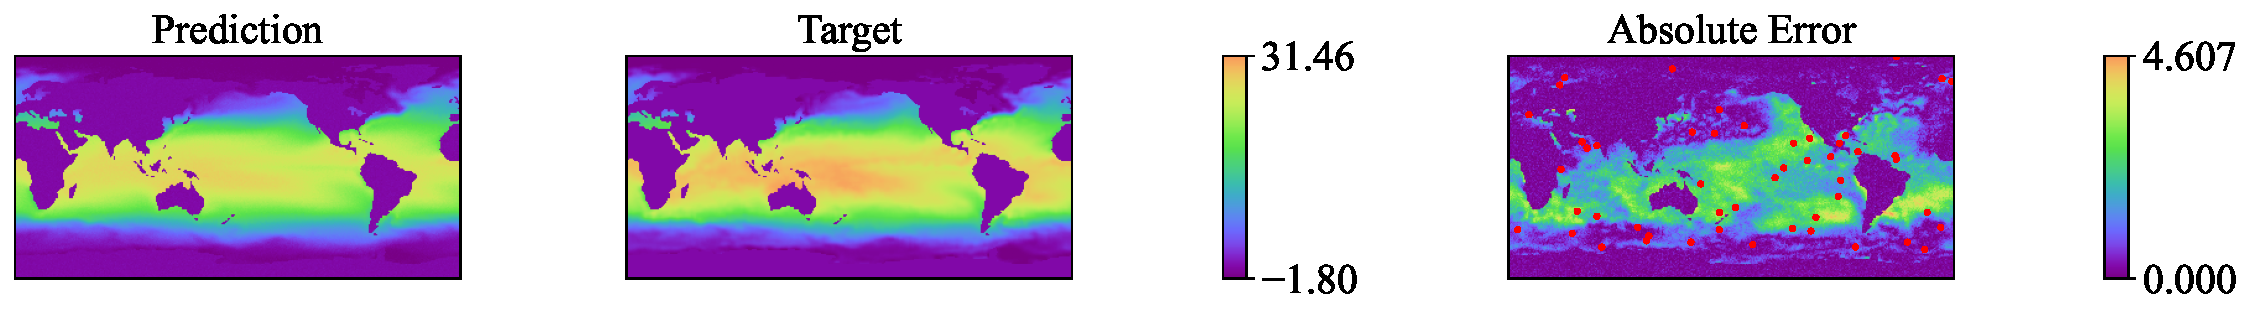
\includegraphics[width=0.95\textwidth]{./Figures/gru_mlp_sst_e1_d1_lr1.00e-02_full_comparison_0.pdf}
        \caption{Predicted vs True Sea-Surface Temperature for the first next-step prediction in the test dataset.}\label{fig:sst_full_0}
    \end{subfigure}
    \begin{subfigure}[t]{\textwidth}
        \centering
        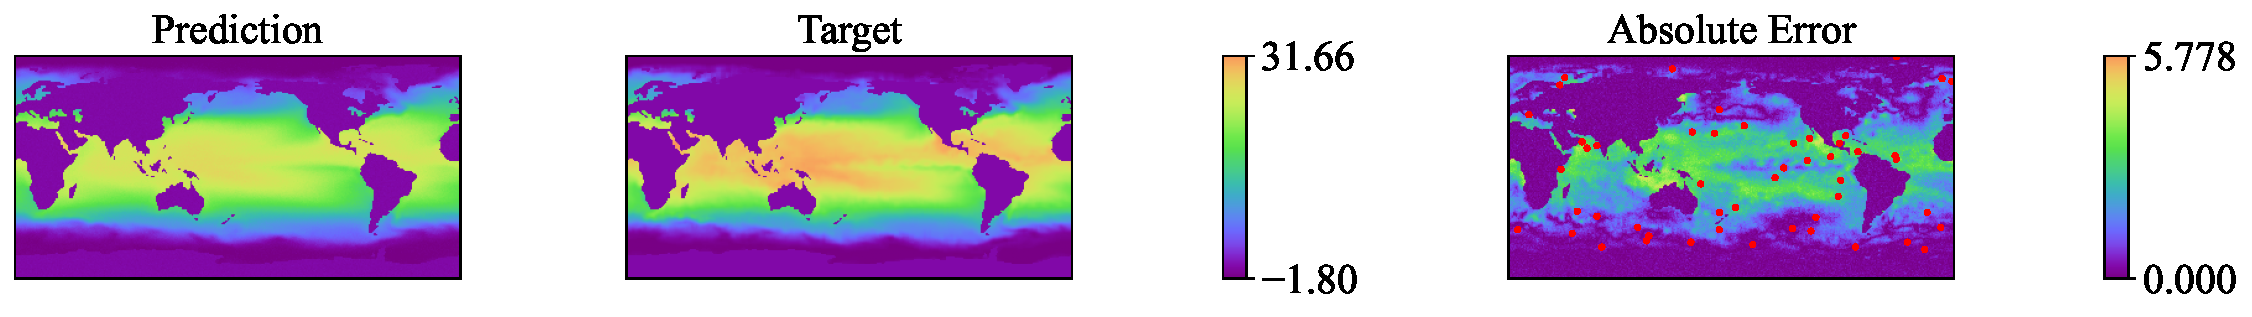
\includegraphics[width=0.95\textwidth]{./Figures/gru_mlp_sst_e1_d1_lr1.00e-02_full_comparison_89.pdf}
        \caption{Predicted vs True Sea-Surface Temperature for the last next-step prediction in the test dataset. Sensor locations are shown in red.}\label{fig:sst_full_89}
    \end{subfigure}
    \caption{Predicted vs True Sea-Surface Temperature for the best performing model on SST (GRU encoder with one layer, UNET decoder with one layer). The top figure shows the next-step state prediction in the test dataset generated by passing first window from the test set and is compared with the true output as well as the absolute error. The bottom figure shows the next-step state prediction in the test dataset generated by passing the last window from the test set and is compared with the true output as well as the absolute error.}\label{fig:sst_full}
\end{figure}

\subsection{Complex Plasma Physics}

% DAVID TODO

The second dataset we consider is the plasma dataset. \textcolor{red}{David: please fill out information about the dataset here.} The data comes as a time-series of 65,792 time-steps where each time-step is represented as a 2,000 dimensional state vector. The dataset's total size is 785MB.

Using the hyperparameters listed above, the top 12 best performing models are shown in \autoref{fig:scatter}

\begin{figure}[H]
\centering
\includegraphics[width=\textwidth]{./Figures/scatter_full.png}
\caption{Top 12 best performing models on each dataset. SL-LSTM representes a SINDy-Loss LSTM, SL-GRU represents a SINDy-Loss GRU, T represents a Vanilla Transformer, SL-T represents a SINDy-Loss Transformer, SA-T represents a Sindy-Attention Transformer, SASL-T a SINDy-Attention SINDy-Loss Transformer.}\label{fig:scatter}
\end{figure}

\begin{figure}[H]
\centering
\includegraphics[width=0.8\textwidth]{./Figures/lstm_mlp_plasma_e3_d1_lr1.00e-02_comparison.pdf}
\caption{Predicted vs True data for the best performing model on the Plasma dataset (LSTM encoder with three layers, MLP decoder with one layer). The left two figures are the predicted and expected states across the full test dataset (not shown is the 50 time-step input window from the test set). The third figure shows the absolute error between the predicted and target states.}\label{fig:plasma_comparison}
\end{figure}

\subsection{Shallow Water Equations}

The third example comes from The Well \cite{ohana2025welllargescalecollectiondiverse}, which a comprehensive collection of numerical physics simulations spanning a diverse set of domains. We use a subset of the \texttt{planetswe} datset from The Well to train our SHRED-based models to observe the performance of T-SHRED in the high-data regime.

The \texttt{planetswe} dataset was generated from simulating the rotating forced hyperviscous spherical shallow water equations:

\begin{equation}
    \frac{\partial \textbf{\textit{u}}}{\partial t} = -\textbf{\textit{u}} \cdot \nabla \textbf{\textit{u}} - g \nabla h - \nu \nabla ^4 \textbf{\textit{u}} - 2 \Omega \times \textbf{\textit{u}}
\end{equation}

\begin{equation}
    \frac{\partial h}{\partial t} = -H \nabla \cdot \textbf{\textit{u}} - \nabla \cdot (h \textbf{\textit{u}}) - \nu \nabla ^4 h + F
\end{equation}

Where $\textbf{\textit{u}}$ is the vector-valued velocity field, $h$ is the surface height, $\nu=1.76 \times 10^{-10}$ was used for simulation stability, and $F$ is a time-dependent forcing term.

To generate our training, testing, and validation data, we first take out the first 10 of the 120 total tracks in the dataset. We then split each of the 10 by taking the first 80\% of the data as training data, the next 10\% of the data as validation data, and the remaining 10\% as the testing data. This results in a total dataset size of 15.5 GB.

The top 12 best performing models trained on \texttt{planetswe} are shown in \autoref{fig:scatter}.

\begin{figure}[H]
    \centering
    \begin{subfigure}[t]{\textwidth}
        \centering
        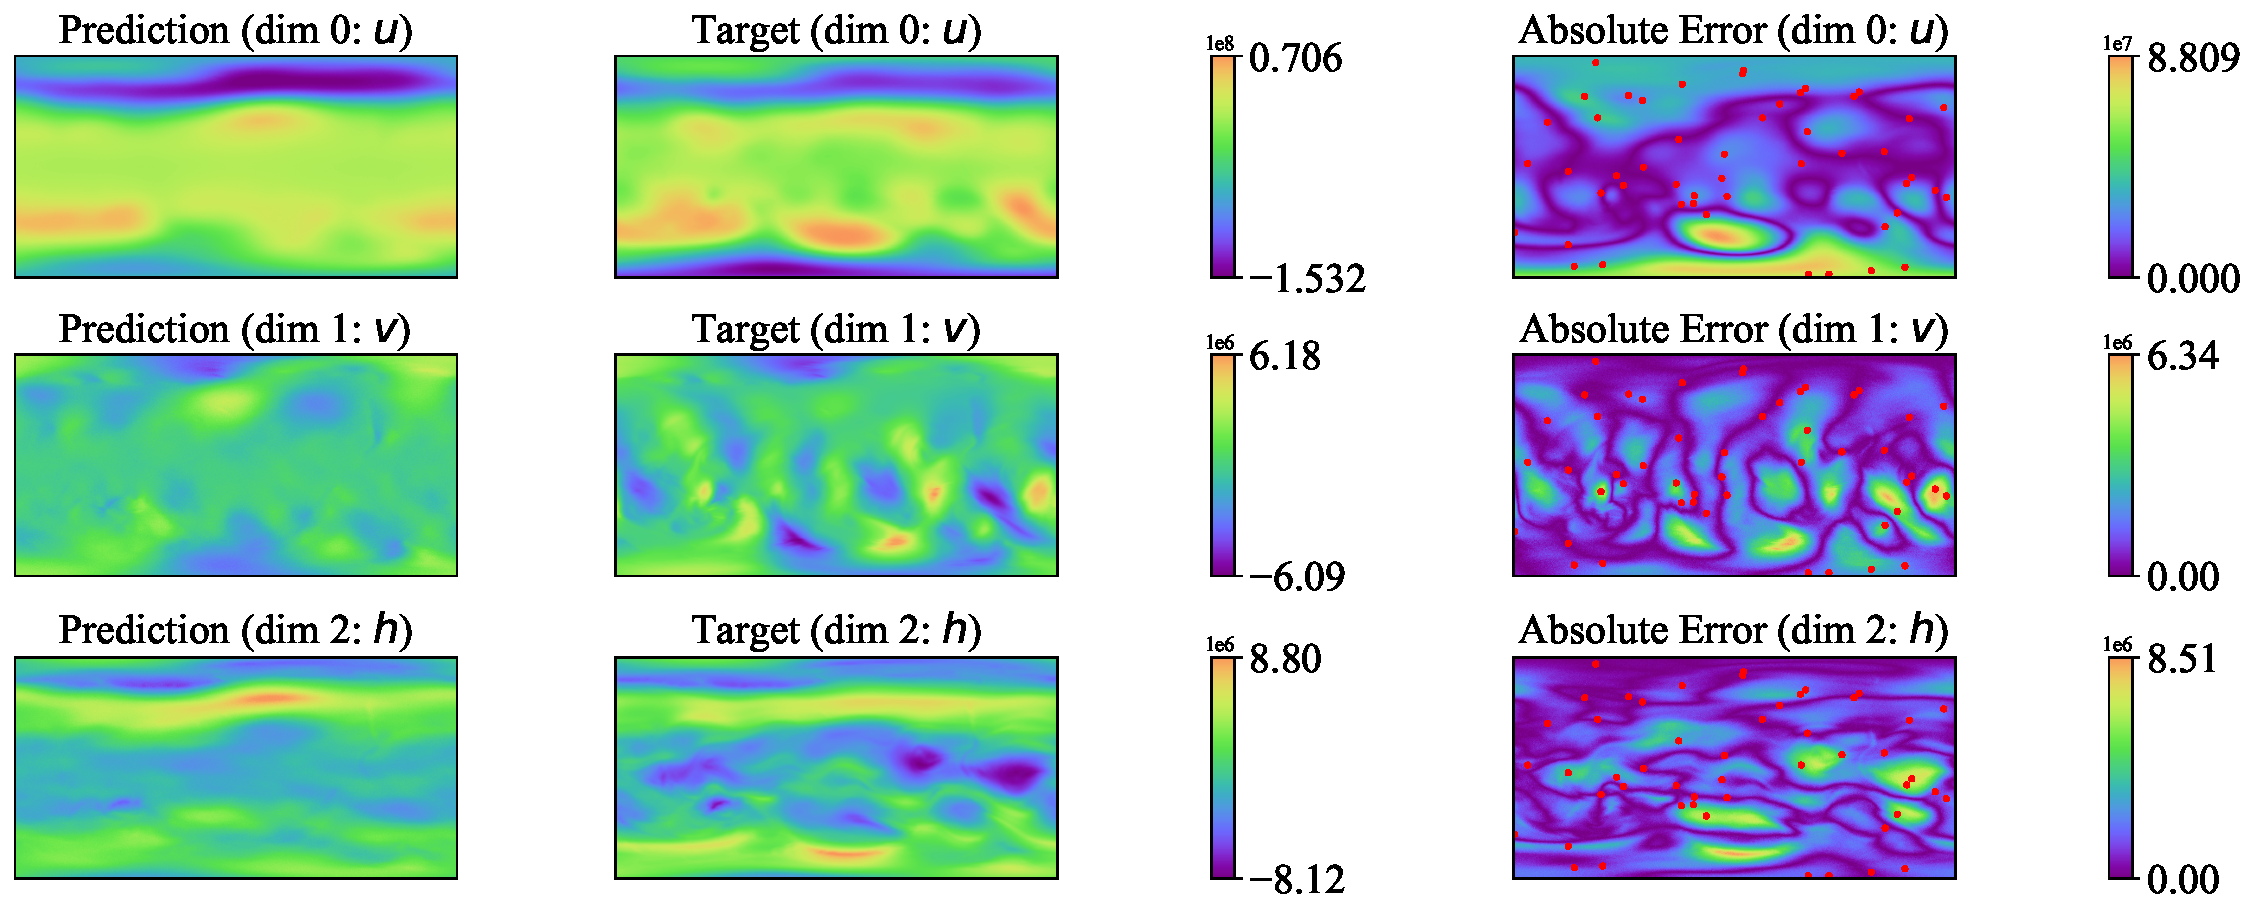
\includegraphics[width=0.95\textwidth]{./Figures/sindy_attention_transformer_mlp_planetswe_full_e4_d1_lr1.00e-03_full_comparison_0.pdf}
        \caption{Predicted vs True PlanetSWE for track 0 for the first next-step prediction in the test dataset. Sensor locations are shown in red.}\label{fig:planetswe_full_0}
    \end{subfigure}
    \begin{subfigure}[t]{\textwidth}
        \centering
        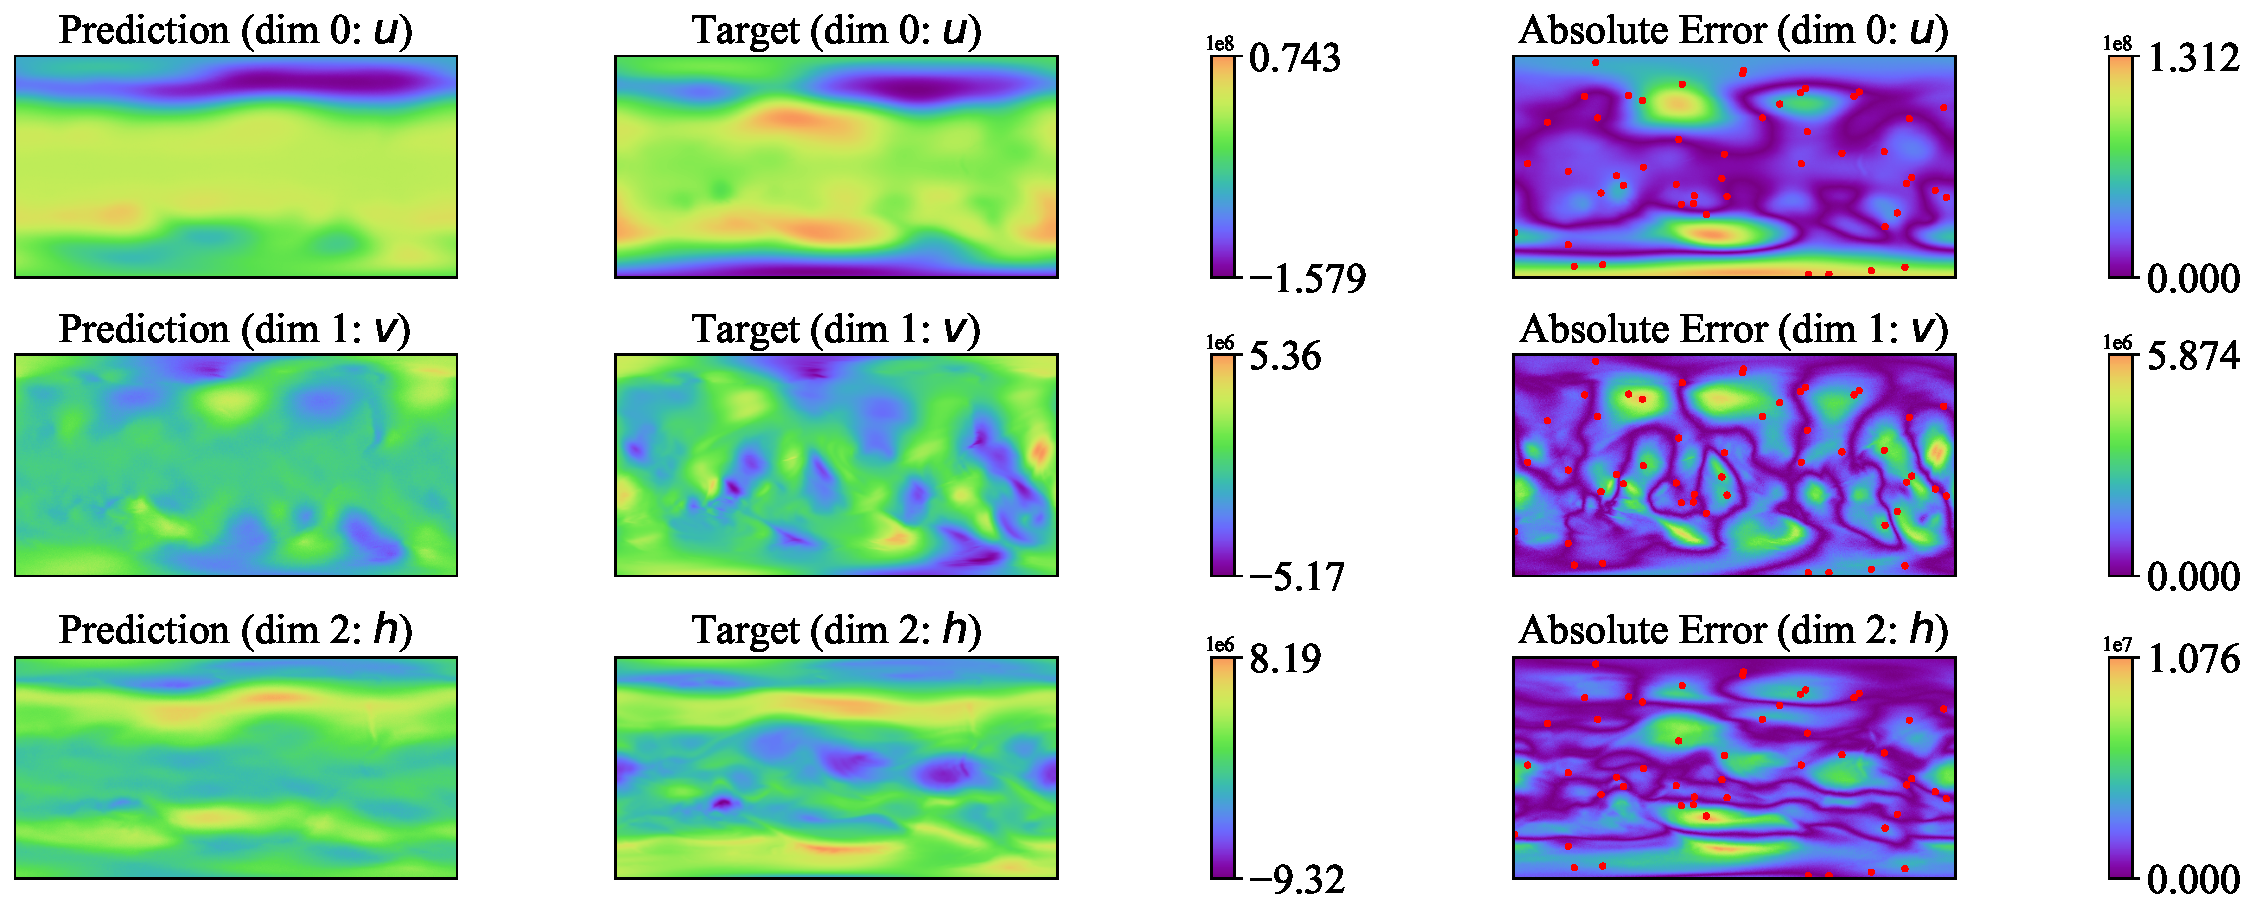
\includegraphics[width=0.95\textwidth]{./Figures/sindy_attention_transformer_mlp_planetswe_full_e4_d1_lr1.00e-03_full_comparison_49.pdf}
        \caption{Predicted vs True PlanetSWE for track 0 for the last next-step prediction in the test dataset.Sensor locations are shown in red.}\label{fig:planetswe_full_49}
    \end{subfigure}
    \caption{Predicted vs True PlanetSWE for track 0 for the first next-step prediction in the test dataset and the last next-step prediction in the test dataset.}\label{fig:planetswe_pod}
\end{figure}

\section{Results}

The experimental results clearly demonstrate that T-SHRED benefits from larger datasets. This aligns with current deep learning literature that use large datasets in their transformer-based architectures to learn complex dependencies in the dataset. Particularly, we observe in \autoref{fig:scatter} RNNs outperform transformers for the low-data regimes of the SST and plasma dataset, with GRUs excelling on SST and LSTMs on the plasma dataset. In contrast, from \autoref{fig:scatter} we see that transformers perform best on the \texttt{planetswe} dataset, comprising all 12 of the lowest test loss models.

Interestingly, while the plasma dataset didn't have any transformers rank in the best 12 lowest test loss models, transformers scored third and fourth in the SST dataset. We also observe that there is no specific transformer configuration that performs better than the rest consistently. The vanilla transformer has just as much of a presence in the high-data regime of \texttt{planetswe} in \autoref{fig:scatter} as with the other models, demonstrating that the core architecture of the transformer is sufficient to learn the underlying dynamics of the dataset. While we do not observe any benefit in using a SINDy attention head or SINDy loss for the final model performance, we do not that the best performing model on \texttt{planetswe} was a SINDy attention transformer paired with a UNET.

We also do not observe any benefit of using either an MLP or a UNET for the SST or plasma datasets; however, it is clear that the top five best performing models on \texttt{planetswe} use UNETs, suggesting their enhanced performance on larger datasets.

\section{Conclusion}

\section{Acknowledgements}

\section{Appendix}

Transformers provide a powerful alternative for sequence modeling.
%
Classical models like RNNs have a limitation in that they have short-term \cite{article}
dependencies associated with exploding and vanishing gradients. For this reason, LSTMs were developed.
LSTMs still struggle with the problem of sequential processing. In other words, LSTMs process input one
sample at a time. This challenge was addressed with bidirectional LSTMs; however, the limitation produced
was contextual loss. Transformers address the concerns regarding sequential processing and contextual loss
\cite{islam2023comprehensivesurveyapplicationstransformers}. By resolving the limitations of RNNs, transformers are said to be more efficient and faster. In addition, the attention mechanism of transformers allows for parallel processing. Parallel processing is a feature
of transformers, whereas RNNs have to process data sequentially.

How do transformers work? The attention mechanism in transformers allows them to process input
sequences in parallel. The attention mechanism was introduced as an approach in computer vision tasks to emphasize certain parts based on their contextual relevance in the application. Incorporating the self-attention mechanism in the transformer model better captured local features and reduced the reliance on
external information. Additionally, transformers possess a positional encoding. Positional encoding provides information as to the order of sequences within the model. In the context of words, the model can
better gauge word order. The reason this is necessary is by processing the data in parallel. The model is not
able to gauge the order of the words. Positional encoding addresses this by encoding the position of each
word within the sequence.

Where are transformers currently applied? Transformers are a neural network model that can learn
representations of sequences or sets of data points. Transformers have driven advances in natural language
processing, computer vision, and spatial-temporal modeling \cite{turner2024introductiontransformers}. For illustration, they have become very
prevalent and well-known in natural language processing. Transformers are useful because, unlike RNNs,
transformers can handle larger input sequences. It is said that transformers have become the predominant
infrastructure and state-of-the-art solution for the majority of learning-based machine intelligence tasks in
the field of artificial intelligence \cite{islam2023comprehensivesurveyapplicationstransformers}. The entire transformer architecture is not used. Instead, the transformer
encoder is utilized \cite{turner2024introductiontransformers}.

What composes the architecture of a transformer?
What are the benefits of utilizing transformers? Transformers address the limitations of preexisting neural
network architectures. They can train faster because they utilize parallel processing. Similarly, transformers
address the vanishing gradient problem, which RNNs have to deal with. In consequence, the transformer can
utilize longer sequences without reduction in training performance. Similarly, as the objective function is
traversed the gradient will not converge too early. Additionally, in biomedical imaging, the transformer can
alleviate the problem of scattered target regions and large shape differences \cite{article}. Similarly, the transformer
can use a convolutional neural network structure to take advantage of the ability of sample information
to extract multiscale local spatial features; this would in turn improve model performance by allowing the
model’s global and local information achieve a balance \cite{article}.

What are the limitations of the transformer architecture? Transformer architectures do have their benefits
that make them very clear to utilize them to build upon SHRED-TUN. However, a limitation of transformers
it that they hallucinate. It is said that a major contribution of this has to do with function composition
\cite{peng2024limitationstransformerarchitecture}. The limitations take place primarily for very large inputs \cite{peng2024limitationstransformerarchitecture}. As an illustration, the issue of function
composition can be explained as such. If you have a sentence, ”Joe’s brother is going for a walk”, brother
relies on the fact that we are referring to Joe. In the context of spatio-temporal data, a hallucination would
be a vastly inaccurate forecasting of the time series that does not match the established ground truth
Y. Despite these limitations, the fact that transformers address the problems of RNNs make them a strong
proponent for utilization in SHRED-TUN.
Why are we using a transformer encoder? The point of this SHRED adaptation (SHRED-TUN) is to be
able to utilize the encoder component of the transformer architecture to capture long-term dependencies in
the time series data. Theoretically, this would make SHRED more generalizable to different problems and
datasets where the temporal connections are longer and more complex. SHRED-TUN is capable of both
forecasting and reconstruction. A transformer encoder allows the whole sequence to be processed in parallel,
which improves the training time of the model. The original SHRED utilizes an RNN encoder. The typical
problems that RNNs face could be resolved using a transformer encoder. The reason for this is that
transformers resolve the typical issues RNNs face. This is relevant because

How does this deviate from SHRED and what is the theoretical result? In theory, SHRED-TUN should
perform better than SHRED because of its ability to capture long-term dependencies / longer sequences
in the data. In this case, better is more generalizable and precise (metric-wise). Moreover, the
utilization of a transformer encoder provides more accurate interpretability than SHRED. The reason for the
improved interpretability comes from the attention-heads of the model. Moreover, this paper will go through \cite{peng2024limitationstransformerarchitecture}
several potential applications of SHRED-TUN that highlight the added interpretability and generalization
of the model. Furthermore, implementing a transformer encoder with SHRED allows the model to
deal with larger datasets more effectively. In principle, the model can scale; more data reduces the model’s
chance to overfit. Consequently, the interpretability and reliability of the model improve. Similarly, the
model does not have to deal with the vanishing gradient problem that RNNs and LSTMs have to deal with because they can look at the whole sequence once due to their self-attention mechanism.
Convolutional neural networks were developed to address certain problems that MLPs faced when dealing with
data that possessed many hierarchical features. Additionally, image data for example possess a large number of pixels, which leads to a significant number of parameters in MLPs that make them computationally
expensive and prone to overfitting. The CNN is a solution to the limitations of the MLP network when
dealing with such data. CNNs have pooling layers that reduce the dimensionality of the data making it less
computationally expensive. Similar to how the development of transformers addressed certain limitations
facing RNNs, the development of CNNs addressed the limitations of RNNs in handling data that would
otherwise produce computationally expensive models.
UNETs are an architecture that was originally developed for biomedical imaging. Their architecture
utilizes skip connections, which has made them useful for tasks where the inputs and outputs have the
same shape. UNets and convolutional decoding have strong evidence in the literature for the ability to
extract features and reconstruct spatial information. UNets have been used in a variety of contexts, such
as image segmentation and signal/image reconstruction. In this paper, the utilization of UNETs provides
the opportunity for SHRED to extract local features better. UNETs rely on convolutional neural networks
as an earlier foundation. In consequence, they are still designed to deal with the limitations of MLPs. The
original SHRED architecture utilized an MLP decoder. In consequence, while effective, it demonstrates that
the utilization of UNETs/CNNs in the SHRED-TUN architecture is reasonable.

What challenges do UNETs overcome? Before UNETs, there were other traditional approaches to image
segmentation in medical imaging. UNETs were designed to overcome the limitations of the traditional
approaches in image segmentation. For instance, UNETs can segment from input-output pairs without user
annotation. User annotation implies sketching image boundaries by hand, which is labor and time-intensive.
Additionally, the fact that the UNET operates only on convolutional layers permits it to work on images
of any size. The encoding path and decoding path of the architecture permit the UNet to learn both global
context and local information. Thus, the UNET architecture is very useful for dealing with reconstruction
tasks that require a model to have the capability to learn different levels of visual information (colors, objects,
etc) similar to a spatial-exploration-based CNN.
The purpose of utilizing UNETs in SHRED is to help the model learn spatial relationships. UNETs excel
at reconstruction in various areas. However, this critical aspect is advantageous for dealing with spatial
and temporal data in a hybrid model such as SHRED-TUN (Shallow Recurrent Decoding with Transformer
Networks and UNETs). SHRED deals with tasks that require a model to learn both local and global
information. Similarly, learning this global features is not sufficient enough. The model must be able to
accurately retain the information with minimal loss to properly reconstruct the data. Similarly, a well-learned
model can better forecast the spatio-temporal data at the respective time steps necessary.

What is the UNet architecture? UNETs consist of two paths as a basic structure. The first path is the
contracting path. The first path provides classification information, and it is also known as the encoder path.
It decreases the spatial dimensions of the images while capturing critical information about the image. The
contracting path utilizes pooling and convolution layers. The second path is known as the decoder path. The
second path consists of up-sampling and concatenations from the contracting path followed by convolutions.
The expansion in the second path allows the network to learn localized classification information. Moreover,
the upsampling allows the model to recover spatial information.
Where are UNETs applied? As stated previously, UNETs have significant applications in medical imaging. This
is due to the recent advances in computer vision within the last decade (U-NETS and its variants for medical
imaging). UNETs are very strong with localization, and UNETs are useful in preserving fine details. This is
helpful in a variety of contexts such as recording EEG signals where fine details are pertinent or reconstructing
images extracted from signal measurements. Additionally, U-NETs are very useful to medical imaging because they create highly detailed segmentation with very limited training samples (U-NET and
6
its variants for medical image segmentation: theory and applications). Another benefit is that U-NETs are
faster to train than other segmentation methods (U-NET and its variants for medical image segmentation:
Theory and applications). Consequently, UNETs/CNNs seemed to be an adequate choice for our decoder
network.

How do UNETs work and why use a UNET decoder? UNETs can be seen as an encoder network followed
by a decoder network in simple terms. The use of a UNET decoder is beneficial. The reason why a UNET
decoder is helpful is that it can recover the spatial relationships from the data rigorously. For emphasis, the
decoder would be useful in capturing the intricacies of the local and global context of the spatiotemporal
data. By using a UNET decoder, SHRED can deal with more complex data and problems. Similarly,
SHRED can improve its reconstruction capacity significantly. This is essential because the original uses
of SHRED are related to reconstruction and forecasting problems. SHRED-TUN as an extension of SHRED
should be able to deal with the problems that SHRED did, but it should be able to do so with significantly
more precision. Additionally, the ability of UNETs to enhance the precision of segmentation or reconstruction
tasks with less data makes it an ideal choice for our network.
SHRED-TUN has many potential uses. This can be seen in the applications section of this paper. The
combination of utilizing transformers and UNETs presents an excellent opportunity for better interpretability
and generalizability to many tasks. SHRED-TUN utilizes a transformer encoder and UNET decoder. The
UNET decoder is a feature that utilizes hyperparameter tuning. In other words, it could be a simple CNN;
it depends on the dataset. In the case of this paper, the UNET-Decoder is a width-based CNN where the
feature maps increase in size at each layer. Additionally, the decoder utilizes same padding across each layer.
SHRED-TUN takes advantage of the transformers resolution of problems regarding RNNs. Furthermore,
SHRED-TUN utilizes the ability of CNNs and UNETs to extract spatial features. SHRED-TUN also deviates
from SHRED in that convolutional neural networks were specifically designed to deal with spatial data such
as images and such. Thus, the SHRED-TUN model theoretically should be an improvement from SHRED
when dealing with data of that context. Moreover, the one-dimensional component of the convolutional
layers are utilized in the process are effective at learning temporal relationships in the data. In this case,
their goal is to decode the spatio-temporal relationships being encoded by the convolutional neural network.
Since the transformer deals with the vanishing gradient problem, SHRED-TUN can utilize
long sequences and more data to provide more effective generalizations to many problems. 

SHRED-TUN has
proven very precise in a myriad of problems/contexts. In similar consideration, the capability of SHRED-
TUN to resolve the vanishing gradient problem seen in SHRED, allows additional information to be retained
in the model. Thus, the reconstruction precision is improved. Since UNETs/CNNs can do more with less
data and transformers allow one to increase the amount of data passed to SHRED with less consequences.
The combination of these two powerful tools provides a relevant jump from SHRED. Since SHRED-TUN
utilizes a transformer encoder, it produces greater interpretability than SHRED. The significance of this is
that it could produce better insights into the patterns for the data it is trained on.
SHRED-TUN can be applied in reconstruction tasks. For instance, the utilization of a UNET in the
SHRED-TUN architecture gives it the possibility to effectively reconstruct spatio-temporal systems that
require the model to learn both global and local information. A possible application of SHRED-TUN would
be a biomedical application given that it utilizes a UNET decoder. SHRED-TUN could be utilized to help
decode MEG signals. Moreover, SHRED-TUN could be utilized to reconstruct relevant features coming from
biomedical signals or images.
Similarly, SHRED-TUN can be used to solve various problems in physics and engineering. An example of
this would be in plasma physics. This work will demonstrate that SHRED-TUN can be effectively utilized
in forecasting and reconstructing plasma signals via multiple sensors. Similarly, SHRED-TUN performs
relatively well when reconstructing plasma signals as well. In consequence, this is a promising application
area for SHRED-TUN. 

For a formulaic representation of the SHRED-TUN architecture referenced in this paper, \text{X $\in$ $\mathbb{R}^{B  \times L \times d_{model}}$}  (batch-size, sequence-length, feature-dim) represents the input to the model. Y represents the output of the model - multi-variable function -, and \text{Z $\in$ $\mathbb{R}^{B \times H_{size}}$} (batch-size, hidden-size) represents the latent dimensions of the encoder. Consequently, the equation for the model assuming four layers can be represented below with two cases - ReLU activation and non-activation. However, we will use represent the equation with four layers. 

\begin{equation}
    Z^{(1)} = TransformerEncoder(X^{(0)})
\end{equation}


\begin{equation}
    Y = \sigma\left(W^{(4)} \cdot \sigma\left(W^{(3)} \cdot \sigma\left(W^{(2)} \cdot \sigma(Z^{(1)}) + b^{(1)}\right) + b^{(2)}\right) + b^{(3)}\right)
\end{equation}


In this work, the metric that was used to measure the performance of SHRED-TUN in both reconstruction and forecasting was root-mean-squared-error. This metric allows one to better
extrapolate the performance of SHRED-TUN relative to the ground truth.
SHRED-TUN, however, does have a limitation. Given the difficulty transformers have with function
composition, SHRED-TUN is limited in how effectively it can forecast signals. However, SHRED-TUN
as the results suggest performs better in reconstruction tasks than forecasting tasks. Beyond this, the
architecture builds upon the SHRED concept and does an excellent job at reconstruction and forecasting
nonetheless. With this in mind, it is critical to benchmark SHRED-TUN with respect to other architectures.
In future work, the limitation of SHRED-TUN may be addressed. If not, latter work will produce an
architecture that extends upon this architecture. Consequently, the performance of the SHRED concept will
continue to improve. With that, the potential of Shallow REcurrent Decoding (SHRED) continues to be
validated. Additionally, future work may focus on testing SHRED-TUN with additional datasets. Given
that this study will test SHRED-TUN on a limited number of datasets. To truly establish an objective of this
paper: generalizability. It will be beneficial to continue this work by testing the architecture on additional
datasets.

\textcolor{red}{Alternative introduction (copied here as a reference)}

The SHRED neural network architecture is demonstrably useful in scientific and engineering applications. Based on the separation of variables technique, the model can be seen as a joint training of learning the temporal trajectory and spatial field of the input data simultaneously through the encoder and decoder respectively \cite{williams2024sensing}. Several works have used SHRED to perform state space reconstruction from a sparse set of sensors in the spatial dimension \cite{williams2024sensing, tomasetto2025reducedordermodelingshallow, gao2025sparseidentificationnonlineardynamics}. These works have shown that a full state reconstruction of the data can be obtained from sparse sensors where the sensors only cover about 0.5\% of the original space. Furthermore, the SHRED models are agnostic to the specific system they are modeling. They can perform Go-Pro physics, where dynamics are learned directly from video \cite{gao2025sparseidentificationnonlineardynamics, tomasetto2025reducedordermodelingshallow}; they can also learn chaotic fluid dynamics from simulations \cite{tomasetto2025reducedordermodelingshallow, gao2025sparseidentificationnonlineardynamics}. These results encourage the further development of SHRED architectures.

While it is clear that the theoretical motivation for SHRED models has led to promising results, previous work has not implemented modern deep learning advancements into the architecture. A significant amount of modern deep learning architectures in every domain use transformers. First used for machine translation \cite{vaswani2017attention}, they utilize a self-attention mechanism to learn complex patterns from large datasets more efficiently than other models available at the time. Since then, significant empirical evidence has been produced showing that transformer-based models scale exceptionally well with more data in a variety of domains and architectures \cite{Zhai_2022_CVPR, kaplan2020scaling, liang2024scaling}. 

In this paper, we introduce Transformer SHRED (T-SHRED) which uses a transformer backbone within the SHRED architecture for sparse sensor modeling. The incorporation of a transformer into the SHRED architecture should outperform previous SHRED models by utilizing recent developments in deep learning. We perform an empirical analysis of T-SHRED with the other SHRED architectures by combining different encoders and decoders and evaluating their performance in next-step full state prediction from a sparse set of measurements. We also study the effect SINDy loss \cite{gao2025sparseidentificationnonlineardynamics} has on our prediction task as well as attaching SINDy onto the individual heads of the transformer.

The next-step state prediction task is performed on three different datasets, all coming from physical phenomena on different scales and with different dataset sizes. We show that as the amount of data used in trainingz SHRED increases, transformer based models outperform traditional Recurrent Neural Network (RNN) SHRED architectures on this task.
\noindent 
\textcolor{red}{Piece of the Introduction}
The SHRED neural network architecture is demonstrably useful in scientific and engineering applications. Based on the separation of variables technique, the model can be seen as a joint training of learning the temporal trajectory and spatial field of the input data simultaneously through the encoder and decoder respectively \cite{williams2024sensing}. Several works have used SHRED to perform state space reconstruction from a sparse set of sensors in the spatial dimension \cite{williams2024sensing, tomasetto2025reducedordermodelingshallow, gao2025sparseidentificationnonlineardynamics}. These works have shown that a full state reconstruction of the data can be obtained from sparse sensors where the sensors only cover about 0.5\% of the original space. Furthermore, the SHRED models are agnostic to the specific system they are modeling. They can perform Go-Pro physics, where dynamics are learned directly from video \cite{gao2025sparseidentificationnonlineardynamics, tomasetto2025reducedordermodelingshallow}; they can also learn chaotic fluid dynamics from simulations \cite{tomasetto2025reducedordermodelingshallow, gao2025sparseidentificationnonlineardynamics}. These results encourage the further development of SHRED architectures.

While it is clear that the theoretical motivation for SHRED models has led to promising results, previous work has not implemented modern deep learning advancements into the architecture. A significant amount of modern deep learning architectures in every domain use transformers. First used for machine translation \cite{vaswani2017attention}, they utilize a self-attention mechanism to learn complex patterns from large datasets more efficiently than other models available at the time. Since then, significant empirical evidence has been produced showing that transformer-based models scale exceptionally well with more data in a variety of domains and architectures \cite{Zhai_2022_CVPR, kaplan2020scaling, liang2024scaling}. 

In this paper, we introduce Transformer SHRED (T-SHRED) which uses a transformer backbone within the SHRED architecture for sparse sensor modeling. We perform an empirical analysis of different SHRED architectures by combining different encoders and decoders and evaluating their performance in next-step full state prediction from a sparse set of measurements. We also study the effect SINDy loss \cite{gao2025sparseidentificationnonlineardynamics} has on our prediction task as well as attaching SINDy onto the individual heads of the transformer.

The next-step state prediction task is performed on three different datasets, all coming from physical phenomena on different scales and with different dataset sizes. We show that as the amount of data used in training SHRED increases, transformer based models outperform traditional Recurrent Neural Network (RNN) SHRED architectures on this task.

\noindent
\textcolor{red}{Alternative Abstract (copied here as a reference)}

Shallow recurrent decoder networks and SINDy-SHRED have succeeded in state estimation and identification with datasets from a myriad of historically challenging tasks. These tasks, in question, pertain to state estimation and identification as well as next-step full state prediction from sparse sensor measurements. Similarly, shallow recurrent decoding as a tool to address the problem of state estimation and identification while providing significant results with limited data has proven successful. State estimation and identification enable further control of complex systems that impact many areas of society that possess functions that are obstructed from view. Thus, these reasons provide the drive to continue pursuing the SHRED concept in SINDy-transformer. The success of the SHRED concept, especially SINDy-SHRED, indicates that it is worth trying to implement the SINDy-Transformer. SHRED provides a baseline for comparison of the performance of the SINDy-Transformer and its theoretical basis. By comparing SINDy-Transformer to historically high-performing models, one can gauge its relevance, functionality, and impact more easily. Additionally, SINDy-SHRED and SHRED utilize RNNs for the encoder. In consequence, this implies it still deals with the vanishing gradient problem. By utilizing a transformer encoder, it is believed that SINDy-Transformer can improve upon the performance of SINDy-SHRED and SHRED, as well as be able to account for situations where there is vast data. In theory, SINDy-Transformer should be able to perform better than SINDy-SHRED and SHRED because of its ability to address the vanishing gradient problem; it should perform better because a large dataset allows the model to learn more complex patterns and generalize better. Similarly, the self-attention capacity of the transformer allows it to process data in parallel and capture long-range spatiotemporal dependencies, which is critical for systems that possess memory. The results in this paper were achieved through experimentation with the SINDy-Transformer indicate that this direction is very promising.

\begin{comment}

\subsection{Gray-Scott Reaction Diffusion}

The Gray-Scott reaction diffusion equations are a set of coupled partial differential equations that describe the change in scalar concentrations of two chemical species A and B in space and time.

\begin{equation}
\frac{\partial A}{\partial t} = \partial_A \Delta A - A B ^2 + f(1-A)
\end{equation}

\begin{equation}
\frac{\partial B}{\partial t} = \partial_B \Delta B - A B ^2 - (f+k)
\end{equation}

The parameters $f$ and $k$ are used to control the amount of species A being added to the system and the amount of species B being removed respectively. The values $\delta_A = 2\cdot10^{-5}$ and $\delta_B = 1\cdot10^{-5}$ were used. The provided dataset contains 154 GB of time-series data: 1200 trajectories, each 1001 steps long, where each step is treated as a 128x128 image with 2 dimensions (the concentrations of species A and B).

% TODO: Do it inline or in a table?

The dataset contains a variety of parameter regimes: $(\text{type}, f, k)$ $\in$ $\{(\text{Gliders},0.014,0.054)$, $(\text{Bubbles},0.098,0.057)$, $(\text{Maze},0.029,0.057)$, $(\text{Worms},0.058,0.065)$, $(\text{Spirals},0.018,0.051)$,\\  $(\text{Spots},0.030,0.062)\}$

\begin{table}[H]
\begin{center}
\begin{tabular}{l|ll}
\hline
        & $f$  & $k$  \\ \hline
Gliders & .014 & .054 \\
Bubbles & .098 & .057 \\
Maze    & .029 & .057 \\
Worms   & .058 & .065 \\
Spirals & .018 & .051 \\
Spots   & .030 & .062 \\ \hline
\end{tabular}
\end{center}
\end{table}

Each of the parameter regimes is simulated for 200 full trajectories, 100 of them are initialized as random Fourier series and 100 of them are initialized with randomly placed Gaussians.

To generate our training, testing, and validation data, we first perform Proper Orthogonal Decomposition on the full dataset to reduce the dimensionality of the dataset. This is necessary since, for a look-back window of $50$, the output dimension of the dataset is $50 \cdot 128 \cdot 128 \cdot 2 = 1,638,400$. To achieve this compression, we concatenate all trajectories and perform randomized Singular Value Decomposition (rSVD) on the full dataset to achieve an approximate factorization of the best $||\cdot||_F$ reconstruction of the data matrix \textbf{A} for a given number of modes $r$ \cite{Eckart_Young_1936}. So, with $\textbf{A} \approx \textbf{U}\ \text{diag}(\textbf{S})\ \textbf{V}^T$ we obtain a low-rank approximation of the dataset $\textbf{A}$ by instead using $\widehat{\textbf{A}} \approx \textbf{A} \textbf{V}$. We further normalize the data by scaling the matrix $\widehat{\textbf{A}}$ to be in the range $[0,1]$. We then split each of the 1200 compressed trajectories, and for each trajectory we take the first 80\% of the data as training data, the next 10\% of the data as validation data, and the remaining 10\% as the testing data.

We use $r=100$ to obtain a low-rank compression of the dataset matrix $\textbf{A}$, $\widehat{\textbf{A}}$, and note that it retains $76.07\%$ of the original dataset ($||A - \widehat{A}||_F = 0.2393$).

Using the hyperparameters listed above, the top 12 best performing models are shown in \autoref{fig:gsdr_scatter}

\begin{figure}[H]
\centering
\includegraphics[width=0.5\textwidth]{./Figures/gsrd_scatter.png}
\caption{Top 12 best performing models on the Gray Scott Reaction Diffusion dataset.}\label{fig:gsdr_scatter}
\end{figure}

\begin{figure}[H]
    \centering
    \begin{subfigure}[t]{0.45\textwidth}
        \centering
        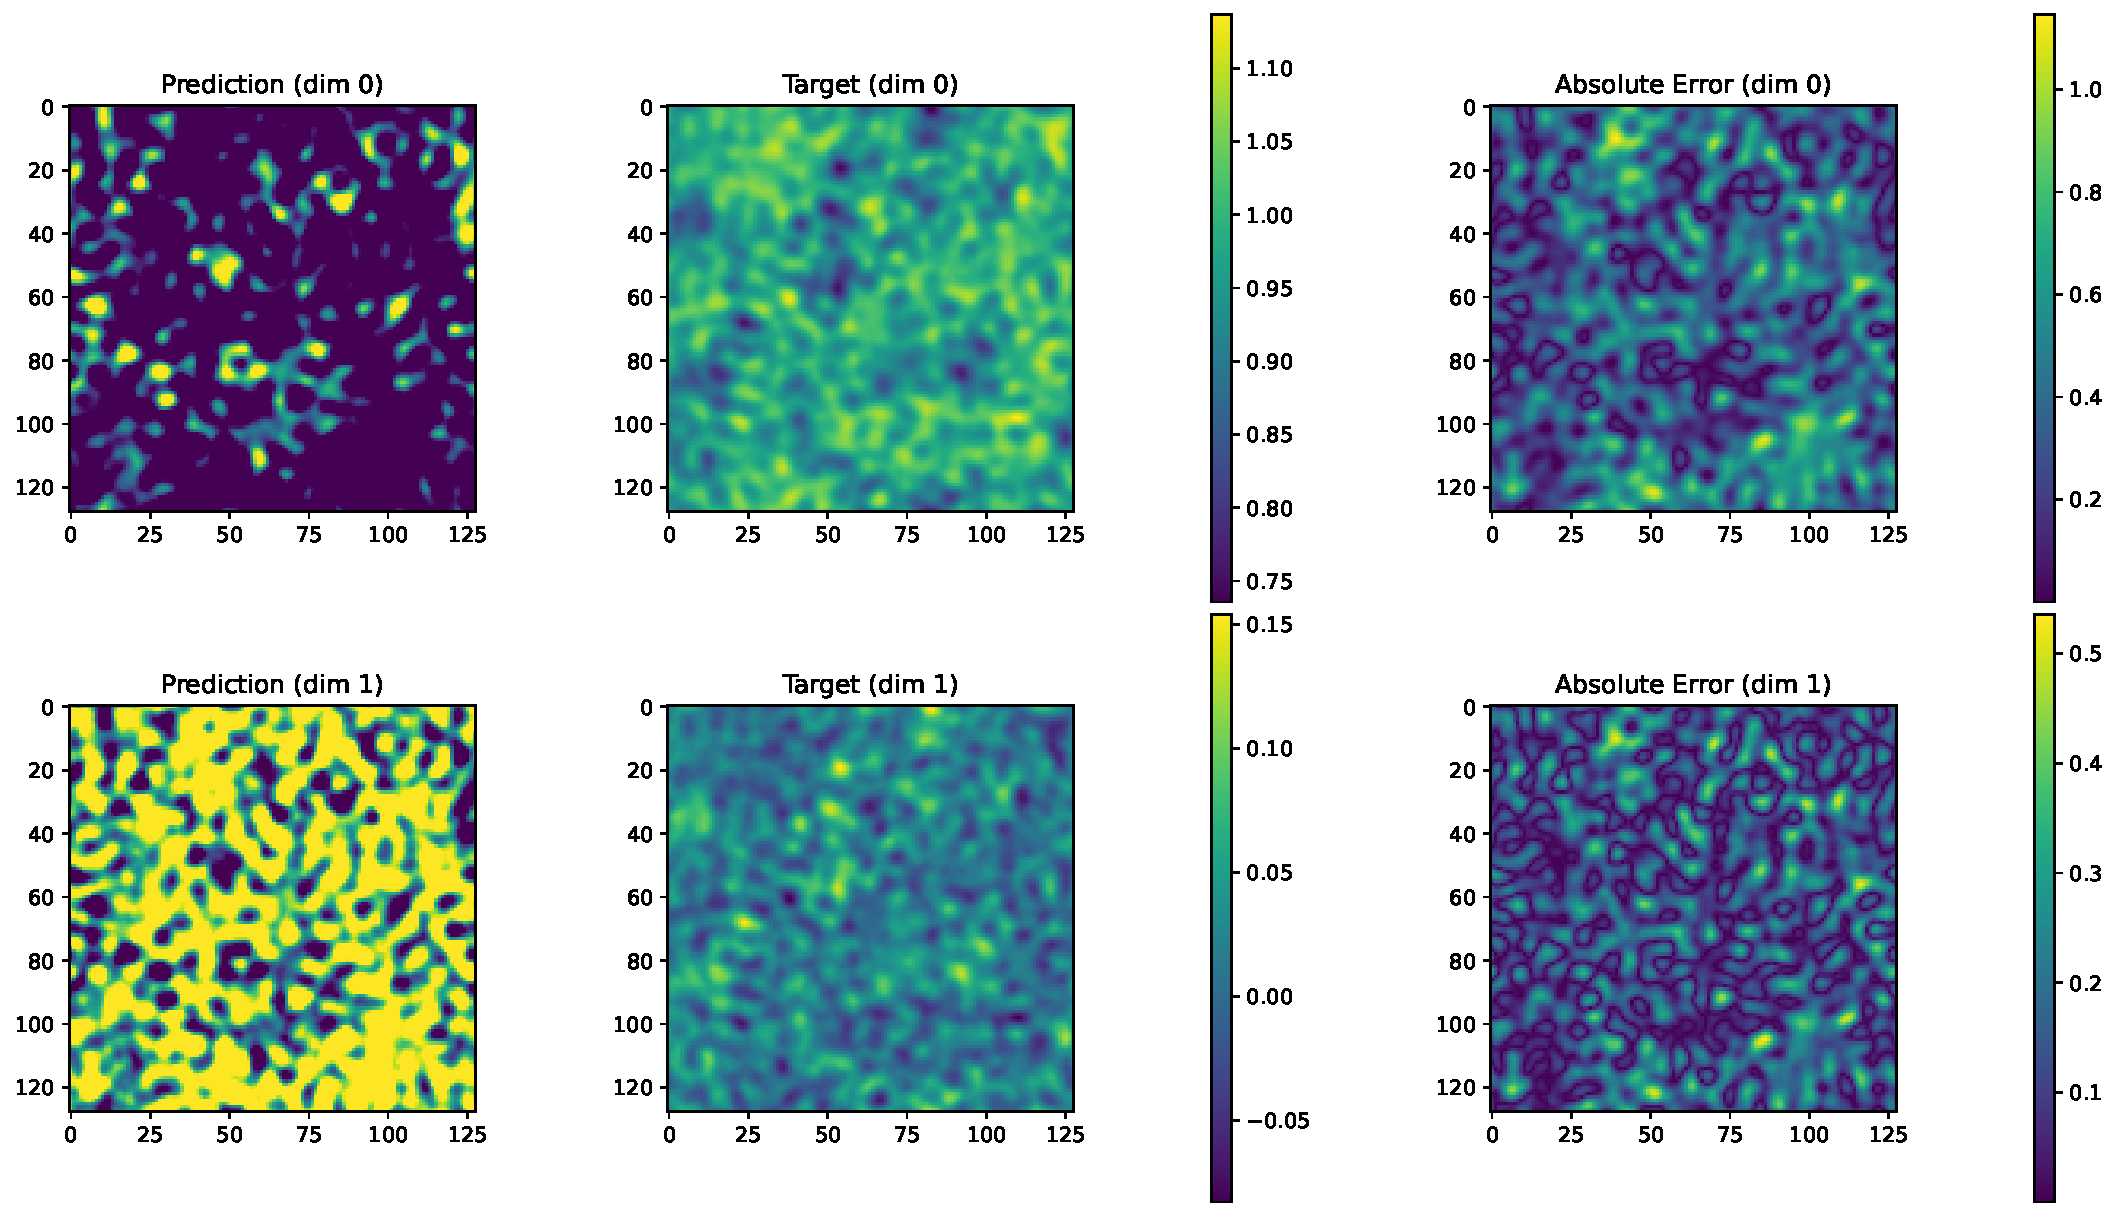
\includegraphics[width=0.95\textwidth]{./Figures/vanilla_transformer_unet_gray_scott_reaction_diffusion_pod_e2_d2_lr1.00e-05_pod_comparison_0.pdf}
        \caption{Predicted vs True Gray-Scott Reaction Diffusion for track 0 for the first next-step prediction in the test dataset (True is POD).}\label{fig:gsdr_pod_0}
    \end{subfigure}%
    ~~~
    \begin{subfigure}[t]{0.45\textwidth}
        \centering
        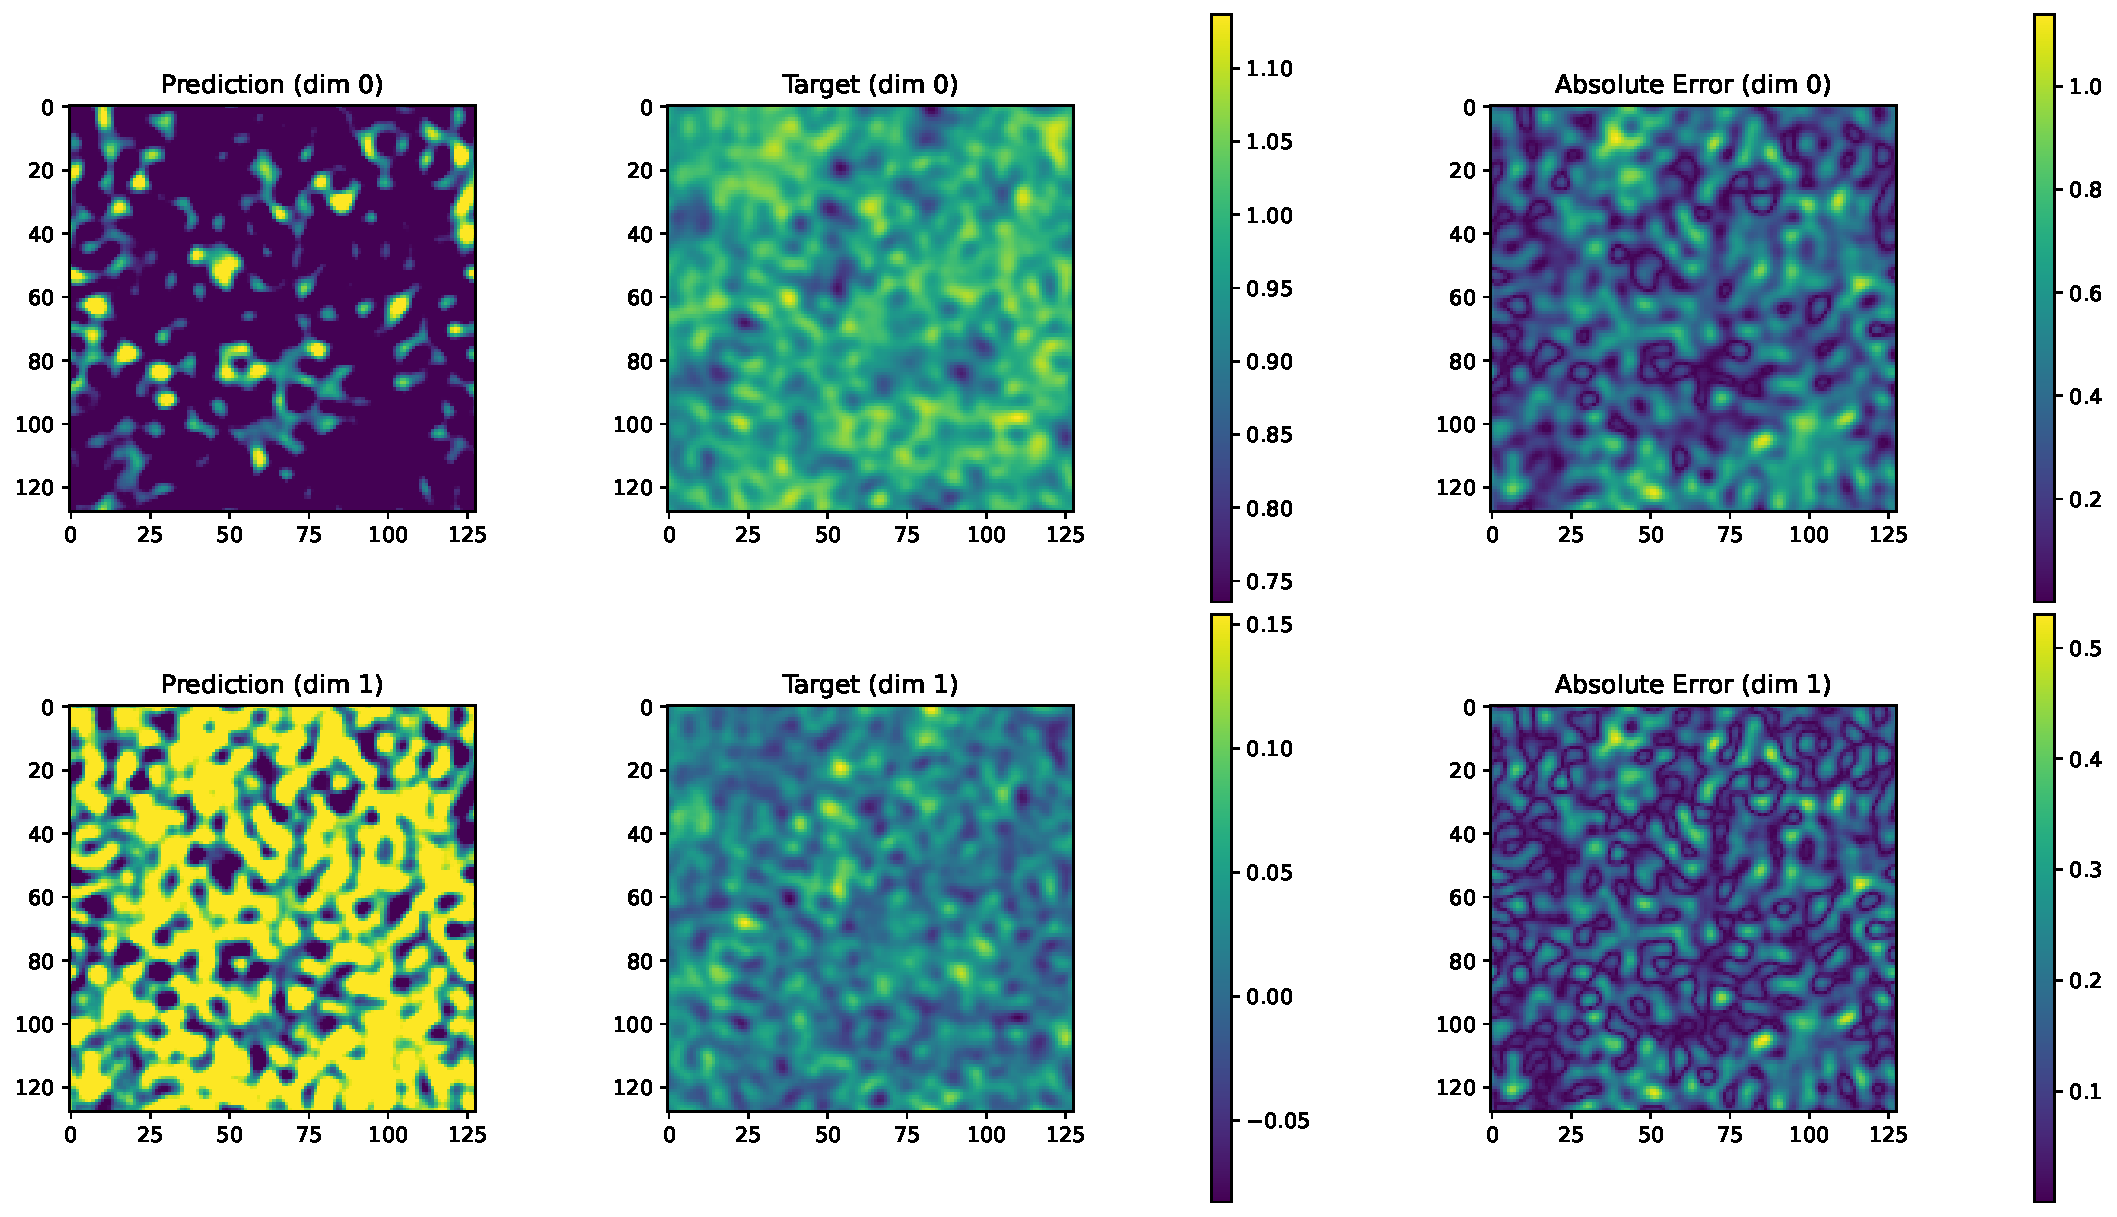
\includegraphics[width=0.95\textwidth]{./Figures/vanilla_transformer_unet_gray_scott_reaction_diffusion_pod_e2_d2_lr1.00e-05_pod_comparison_49.pdf}
        \caption{Predicted vs True Gray-Scott Reaction Diffusion for track 0 for the last next-step prediction in the test dataset (True is POD).}\label{fig:gsdr_pod_49}
    \end{subfigure}
    \caption{Predicted vs True Gray-Scott Reaction Diffusion for track 0 for the first next-step prediction in the test dataset and the last next-step prediction in the test dataset.}\label{fig:gsdr_pod}
\end{figure}

\begin{figure}[H]
    \centering
    \begin{subfigure}[t]{0.45\textwidth}
        \centering
        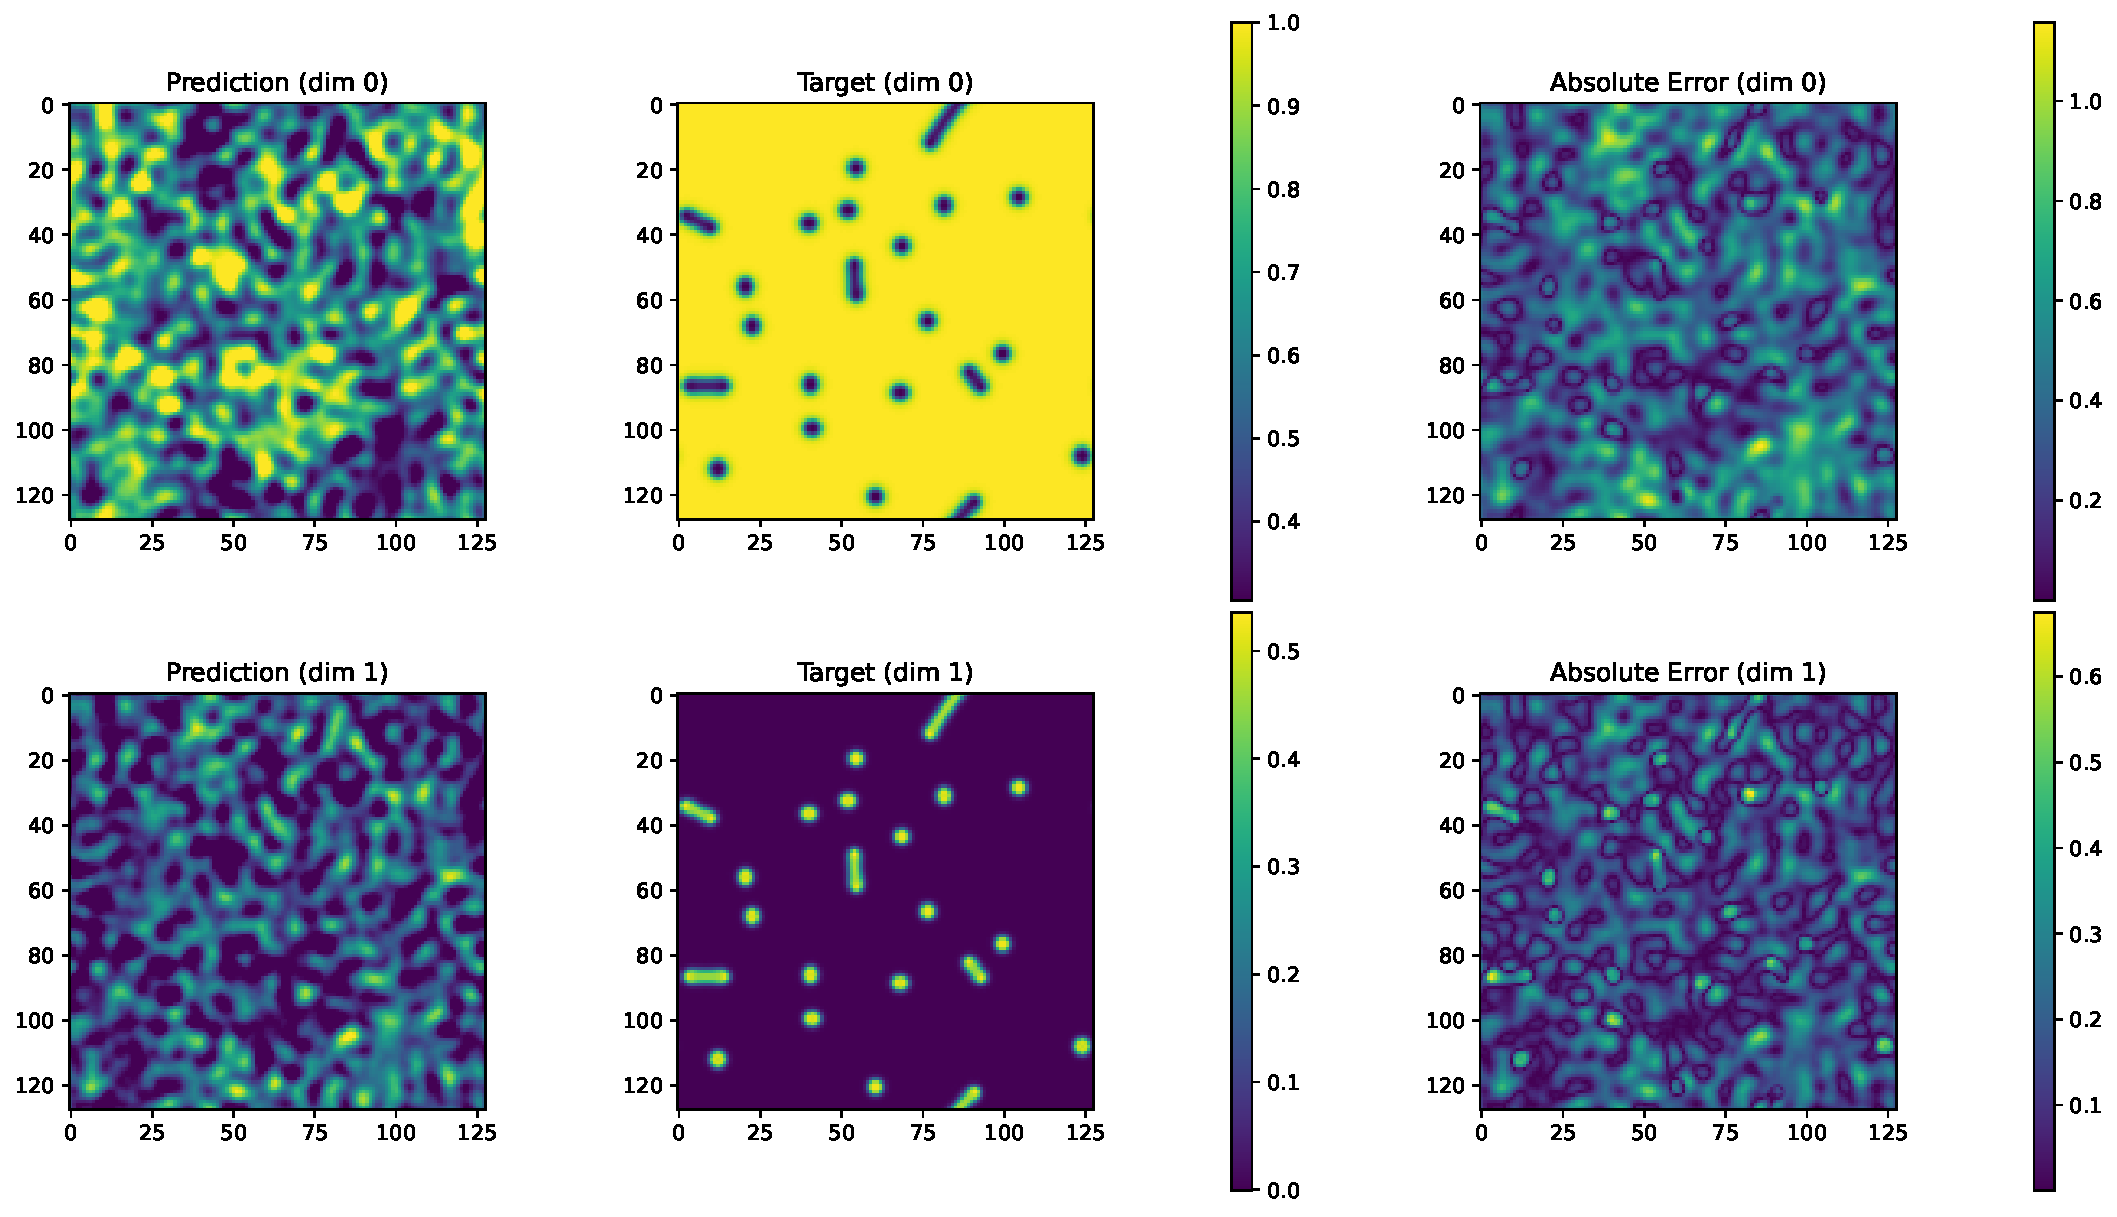
\includegraphics[width=0.95\textwidth]{./Figures/vanilla_transformer_unet_gray_scott_reaction_diffusion_pod_e2_d2_lr1.00e-05_full_comparison_0.pdf}
        \caption{Predicted vs True Gray-Scott Reaction Diffusion for track 0 for the first next-step prediction in the test dataset.}\label{fig:gsdr_full_0}
    \end{subfigure}%
    ~~~
    \begin{subfigure}[t]{0.45\textwidth}
        \centering
        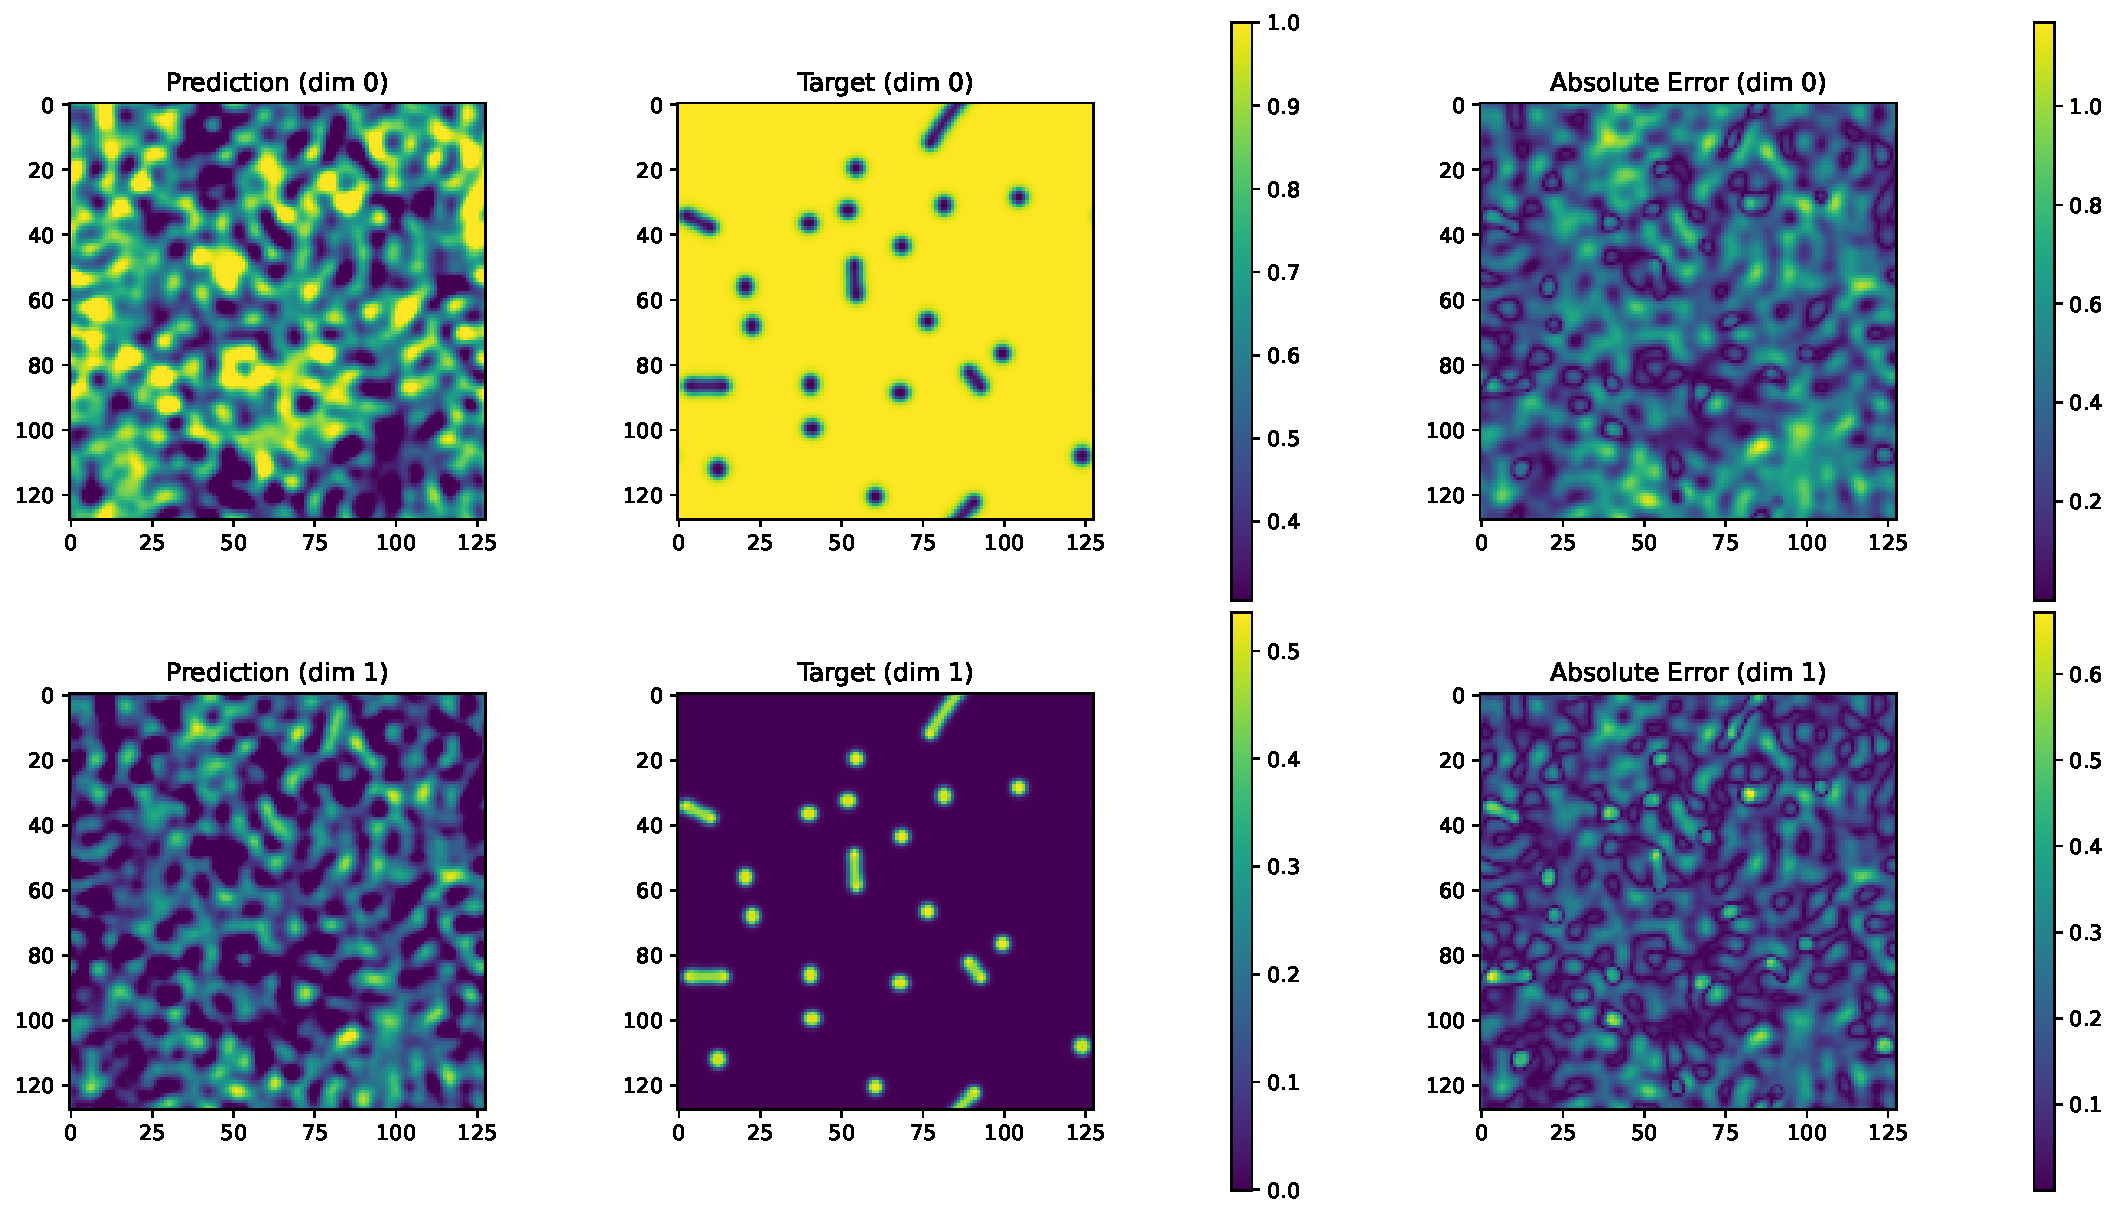
\includegraphics[width=0.95\textwidth]{./Figures/vanilla_transformer_unet_gray_scott_reaction_diffusion_pod_e2_d2_lr1.00e-05_full_comparison_49.pdf}
        \caption{Predicted vs True Gray-Scott Reaction Diffusion for track 0 for the last next-step prediction in the test dataset.}\label{fig:gsdr_full_49}
    \end{subfigure}
    \caption{Predicted vs True Gray-Scott Reaction Diffusion for track 0 for the first next-step prediction in the test dataset and the last next-step prediction in the test dataset.}\label{fig:gsdr_full}
\end{figure}


\end{comment}

\section*{References}
\bibliographystyle{unsrtsiam}
\bibliography{refs}

\end{document}